\documentclass[15pt,twoside]{report}



\usepackage[a4paper,width=150mm,top=25mm,bottom=25mm,bindingoffset=6mm]{geometry}

\usepackage[utf8]{inputenc}
\usepackage{graphicx}
\usepackage{float}
\usepackage{fancyhdr}
\usepackage[nohyperlinks, printonlyused, withpage, smaller]{acronym}
\usepackage[sorting=nyt,backend=biber,style=authoryear]{biblatex}
\usepackage[inkscapeformat=png]{svg}
\usepackage{booktabs,multirow,array}
\usepackage{listings}
\usepackage{xcolor}
\usepackage{amsmath}

\usepackage[font=small,labelfont=bf,tableposition=top]{caption}
\usepackage{tikz}
\usepackage{tocloft}
\usepackage{enumitem}
\usepackage{appendix}

\usetikzlibrary{positioning}
\captionsetup[table]{skip=5pt}

% Customize list of figures appearance in table of contents
\renewcommand{\cftfigpresnum}{\figurename\ }
\setlength{\cftfigindent}{0pt}
\setlength{\cftfignumwidth}{6.5em}


\definecolor{codegreen}{rgb}{0,0.6,0}
\definecolor{codegray}{rgb}{0.5,0.5,0.5}
\definecolor{codepurple}{rgb}{0.58,0,0.82}
\definecolor{backcolour}{rgb}{0.95,0.95,0.92}




% Define the page style "mystyle" for the fancyhdr package
\fancypagestyle{mypagestyle}{
     % Clear all header and footer fields
     \fancyhf{}
     % Set the header to display the chapter name on the right side
     \fancyhead[R]{\leftmark}
     % Set the footer to display the page number on the center
     \fancyfoot[C]{\thepage}
     % Set the footer line to appear (change 0pt to desired line thickness)
     \renewcommand{\footrulewidth}{0.4pt}

}

\lstdefinestyle{mystyle}{
    backgroundcolor=\color{backcolour},   
    commentstyle=\color{codegreen},
    keywordstyle=\color{magenta},
    numberstyle=\tiny\color{codegray},
    stringstyle=\color{codepurple},
    basicstyle=\ttfamily\footnotesize,
    breakatwhitespace=false,         
    breaklines=true,                 
    captionpos=b,                    
    keepspaces=true,                 
    numbers=left,                    
    numbersep=5pt,                  
    showspaces=false,                
    showstringspaces=false,
    showtabs=false,                  
    tabsize=2
}

\lstset{style=mystyle}

\graphicspath{ {images/} }

\renewbibmacro*{url+urldate}{%
  \printfield{url}%
  \iffieldundef{urlyear}
    {}
    {\setunit*{\addspace}%
     \printtext[urldate]{\printurldate}}}

\DeclareFieldFormat{url}{Available at\addcolon\space\url{#1}}

\DeclareFieldFormat{urldate}{\\Accessed on\addcolon\space#1}

\addbibresource{References.bib}

\includeonly{preliminary/title, %
preliminary/affidavit, %
preliminary/abstract, %
preliminary/acronyms, %
chapters/introduction, %
chapters/taxonomy-background, %
chapters/chapter2,%
chapters/chapter3,%
chapters/chapter4,%
chapters/chapter5,%
chapters/chapter6,%
chapters/chapter7,%
chapters/chapter1,%
chapters/conclusion, %
chapters/appendix%
}

\begin{document}


%--------------- Prelimanary pages -------------


%--------------------------------------------
\begin{titlepage}

    \vspace*{3\baselineskip}
        \begin{flushright}        
  
                
\includegraphics[scale=0.3]{SRH_Hochschule_Heidelberg_logo.svg.png}
           
        \end{flushright}
    \vspace*{3\baselineskip}

    \centering
   


    {\Large \bfseries Application of Natural language processing in E-Commerce \\ Predicting product taxonomy}
    \vspace*{3\baselineskip}

    {\Large Master Thesis}
    \vspace*{1\baselineskip}

    {\Large by }
    \vspace*{2\baselineskip}

    {\Large  \bfseries Shoney Arickathil }
    \vspace*{0.5\baselineskip}

    {\Large  Student no: 11017678 }
    \vspace*{2\baselineskip}

    {\Large \today}
    \vspace*{8\baselineskip}

    % \includegraphics[width=0.35\linewidth]{srhlogo}

    {\Large  Masters in Applied Computer Science }
    \vspace*{0.5\baselineskip}

    {\Large  SRH University Heidelberg \\ School of Informatics}  
    \vspace*{6\baselineskip}

    \begin{minipage}{\textwidth}
        \begin{flushleft} % Left-align supervisor's name
            \large Primary Supervisor: \hfill \bfseries Prof. Dr. Gerd Moeckel
           
        \end{flushleft}
       
       
    \end{minipage}

    


   
    
\end{titlepage}

\begin{titlepage}
    \begin{flushright}
        
  
\section*{Declaration}
\justifying {
I hereby declare that the work presented in this Project Report titled \textbf{ Machine Learning for traffic flow prediction at different junctions – M.Tech}. Submitted to the \textbf{ Indian Institute of Technology Jodhpur} in partial fulfilment of the requirements for the award of the degree of M.Tech (Masters of Technology), is a Bonafide record of the research work carried out under the supervision of \textbf{ Dr. Ranju Mohan}. The contents of this Project Report in full or in parts, have not been submitted to, and will not be submitted by me to, any other Institute or University in India or abroad for the award of any degree or diploma.
}
\vspace*{3\baselineskip}


{\large \bfseries Cyril John Arickathil \par}
{\large \bfseries M22RM210 \par}


\end{flushright}

\end{titlepage}

\begin{abstract}
    

\begin{center}
    Shoney Arickathil, School of Informatics, SRH Hochschule Heidelberg \\

Master Thesis \\
\textbf{Application of Natural language processing in ECommerce}\\
\textbf{Predicting product taxonomy}

\end{center}


Electronic commerce started in early 1990's in which the business transactions are conducted through computer networks. The ease of buying a product online has reduced physical work and time required for decision-making by compare the product features. A wide range of products are sold online. One of the challenge is to well define a products' taxonomy. A product taxonomy is a hierarchical structure to organize the products in an E-commerce platform in such a way that customers can find the product in the fewest possible clicks.
Product taxonomy for the same product may differ based on the supplier and manufacturer (sources). Hence, product taxonomy details cannot be imported directly from the sources into the E-commerce platform. Product details cannot be live until its taxonomy is not well-defined, this delays the time of product availability for customers. 

In this thesis the author developed a machine learning classification model to predict the product taxonomy based on the features of the product. This is achieved with machine learning model. Experimenting and analyzing by varying  model's parameters facilitated to determine models performance.  

Initially, from the existing product taxonomy the features such as name and description were extracted. These extracted features were passed through process of text normalization, imputation of missing text to standardize it before converting it into One-Hot encoded format. These features and its lowest hierarchical level of category were processed by \acf*{RNN} machine learning model to learn the patterns of feature and classify it with the concept of probability distribution.

The result of predicting the lowest hierarchical level of product category based only on product name formed a foundation to create a machine learning model to predict the complete product taxonomy. As the level of category to be predicted increases the model's weight and product features need to be adjusted. 

\end{abstract}





\pagenumbering{roman}
\pagestyle{plain}
\tableofcontents

\clearpage
%----------------- chapters --------------------
\pagestyle{mypagestyle}
\pagenumbering{arabic}

%---------------------------------------
\chapter{Introduction}

\section{Topic overview}


\chapter{Literature Review}

\section{E-commerce and Product Taxonomy}

A product taxonomy is a hierarchical representation of product catalog organized logically so that the customer can find the product in the fewest possible clicks. The top levels of hierarchy are general terms and low levels are narrowed down to specific and semantically closer to the product.  


Product taxonomy can be represented as a directed acyclic graph. The top level of root node traversing below to leaf nodes connected with unidirectional edges representing relationship between the nodes. 


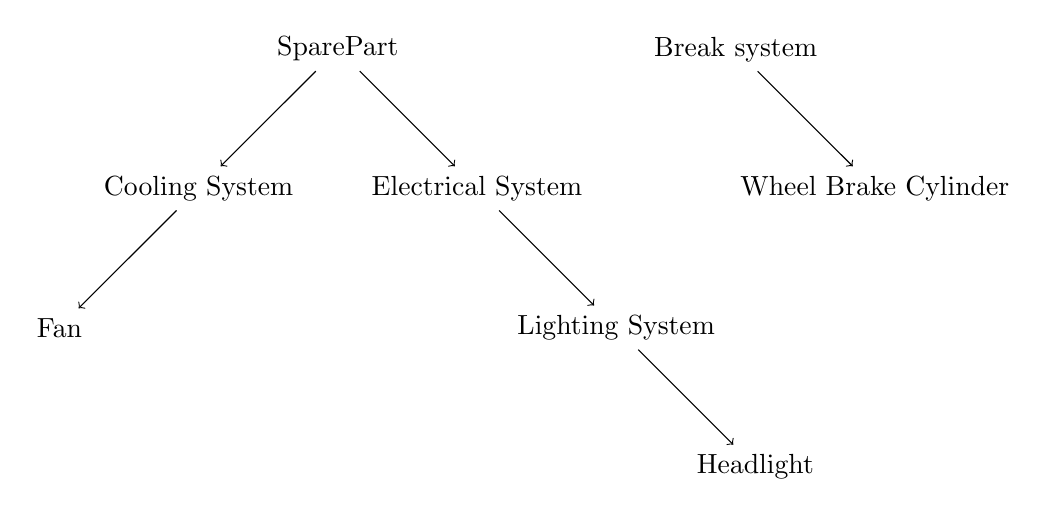
\begin{tikzpicture}[node distance=2.5cm]
    % Nodes
    \node (sparepart) {SparePart};
    \node (break-system)[right=3cm of sparepart] {Break system};
    \node (cylinder-head)[below right of=break-system] {Wheel Brake Cylinder};
    \node (coolingsystem) [below left of=sparepart] {Cooling System};
    \node (fan) [below left of=coolingsystem] {Fan};
    \node (electricalsystem) [below right of=sparepart] {Electrical System};

    \node (lightingsystem) [below right of=electricalsystem] {Lighting System};

    \node (headlighgt) [below right of=lightingsystem] {Headlight};
    
    % Arrows
    \draw[->] (sparepart) -- (coolingsystem);
    \draw[->] (coolingsystem) -- (fan);
    \draw[->] (sparepart) -- (electricalsystem);
    \draw[->] (electricalsystem) -- (lightingsystem);
    \draw[->] (lightingsystem) -- (headlighgt);
    \draw[->] (break-system) -- (cylinder-head);
  \end{tikzpicture}
 
 
  What are the characteristics of this sample of product taxonomies?
\begin{itemize}
    \item Product taxonomy has different lowest levels of hierarchy. For example, category ``Fan'' is at third level and ``Headlight'' being a part of ``Electrical Systems'' is at fourth level.
    \item Few categories having similar vocabulary are part of same graph. For example, category with the word ``Brake'' are connected with the edges.  Similary, the category ``Lighting system'' and its leaf node ``Headlight'' share a same semantically meaning word ``light''.
    \item The root nodes ``Sparepart'' and ``Break system'' are isolated from each other, indicating that they do not have any common entity. 
    \item The node ``Break system'' could also be a part of node ``Sparepart'' and yet the taxonomy will remain well-defined as it is a general term.
\end{itemize}

These enlisted characteristics could be an insight on developing an automated product taxonomy.

How important is a well-defined product taxonomy?
\begin{itemize}
    \item Customer filters the category to narrow down the search result, enabling them to find the required product in the fewest possible clicks.
    \item Product recommendation system analyze the purchase history of customer and returns the related products. A well-defined product taxonomy is important for mapping the related products.
\end{itemize}

\section{Product Taxonomy Prediction Approaches}


A lot of research have been conducted on methodology for predicting taxonomy. Prediction of taxonomies narrows down to text classification. Text classification is a process of identifying the group or category in which the  text belongs to.  Few classification methods are decision trees, naive Bayes classifier and max entropy classifiers \parencite{BirdKleinLoper09}. 


\begin{itemize}
    \item Decision  tree
    
    A decision tree is a flowchart that selects labels for input values. This flowchart consists of decision nodes, which check feature values, and leaf nodes, which assign labels. 

    \item Naive Bayes classifiers
    
    In naive Bayes classifiers, each feature values determining which label should be assigned to a given input value. It begins by calculating prior probability of each label. It is determined by frequency of each label in the training set. Upon combining these prior probability, the likelihood estimation is calculated for each label. The with the highest likelihood estimate is assigned to the input values.
\end{itemize}

\section{Related work}

\parencite{AliCevahir.} describes implementing classification model by chunking the process to predict at every level using the \acl*{KNN} classifier. \parencite{Gupta.20062016}  proposes a distributional semantics representation for predicting the product taxonomies.





\chapter{Prerequisites for developing classification model}

One of the major challenge in an ecommerce industry is to categorize the products. The phenominal types of products in the ecommerce web application sold online may require an artificial inteligence generated category tree. The multi level product-categories in the taxonomy tree received and defined from the suppliers or manfucture may not be usable. Since the existing multi level category of those products in ecommerse application may defer. Importing product-category details directly from the various channels may lead to disambugution. The artificial inteligence generated category tree reduces the product ready to deploy time on the production environment. The product ready to deploy time here refers to the check lists of data correctness of the product before listing online.

\section {Fetch existing product taxonomy using Elastic Search}

In section \ref {pyenv}, version specific python client installation detail are documented. For this project, python client elasticsearch 6.8.2 is installed as the client needs to be compatble with Elastic search version being used.


\begin{lstlisting}[language=Python]
from elasticsearch import Elasticsearch
client = Elasticsearch("http://localhost:9200")

resp = client.search(index="development_products",
                     body={"_source":["descriptions","descriptionsSource","nameSource","shortDescriptionSource","categoriesSource"],
                           "query": {"match_all": {}}})
\end{lstlisting}

The above code sample fetches the features of the product such as "name","description",category".


Elasticsearch uses \acf{Tf-Idf}. \acs{Tf-Idf} is a technique to generate numeric representation of words. \acs{Tf-Idf} represents product of two terms, \acs{Tf} and \acs{Idf}.

% \begin{math} x_i=tf(w_i) x idf(w_i) \end{math}

\section {Feature selection and dataset sources}

A feature represents a set of data inputed in a training model to predict the the masked related data. In simple terms, in a classication model which predicts category of a product, product name, description can be labeled as its feature. 

The datasets used primarly for extracting feautures will be from the existing product database. In this paper, the datasets used are of an ecommerce business belonging to automotive industry domain. Secondary dataset used is from the TecDoc catalogue by TecAlliance \footnote{https://www.tecalliance.net/}

 In this experiment, consider 5 levels of categories as the maximum limit. The number of category levels differ for each products. Consider an example of category tree with three levels. 

\begin{quote} 
\centering 
sparepart/cooling-system/thermostat
\end{quote}
In such case, level 4 and level 5 will be appended with values using data imputation techniques, refer section \ref{dataimput}. 

The table \ref{table:l5} lists the feature description aling with the sample of category levels.
% \begin{figure}[h]
%       \centering
%       \small{This is text.  It's in a figure environment but it's still text}
%       \caption{\label{fig_text}Some text that can float as a figure}
%   \end{figure}



\begin{table}
      \caption{Feature descriptin and five levels of category sample data}
      \label{table:l5}

% \end{table}

% \begin{table}
%       \caption{Feature descriptions}
%       \label{table:features}
      \begin{tabular}{ lll }
            \toprule
            
            \textbf{No}& \textbf{Feature} & \textbf{Value}\\
            \midrule
            1&Category tree & multi level categories\\
            2&Description & description with html tags\\
            3&Manufacturere & name of company manfactured\\
            4&Short description  & product info displayed\\
            5&Supplier  &  supplier of the product\\
            \color{red}6&n number of  category levels   &  feature extracted from category tree\\
           
            \bottomrule
            \end{tabular}

            \begin{tabular}{llllll}
                  \toprule
                   catlevel0 & catlevel1 & catlevel2 & catlevel3 & catlevel4 & catlevel5 \\
                  \midrule
                  sparepart & cooling system & thermostat & NaN & NaN & NaN \\
            
                  \bottomrule
            \end{tabular}

\end{table}


\subsection{Dependency parsing for extracting nouns from features}

\section {Data imputation techniques - on missing data} \label{dataimput}

\subsection {Forward and Backward fill}

\subsection {Impute with mode}
\chapter{Text normalization} \label{text_normalization}

Text normalization is a process of transforming the document into a standard and consistent form of a text. A document is a text from single source. Some examples of document are list of product names from databases, a pdf file, texts retrieved from web scraping. Text normalization enables to perform required operations on the text as the text inputs are consistent across the document. The process of text normalization varies based on the type of text that needs to normalize. There is no standard method for text normalization task. In this paper, text normalization of product name and category from the database source is performed. The text are of two languages, English and Deutsche.

In table \ref{table:TN}, displays the difference in text before and after normalization. 

\begin{table}[h]
      \caption{Sample of text normalization effect}
      \centering
      \label{table:TN}
\begin{tabular}{lll}
      \toprule 
                  &\textbf{Name} & \textbf{Category} \\ 
      \midrule
      \textbf{Before}&VAICO V10-4245 Stoßdämpfer & Stoßdämpfer \\
      \textbf{After}&vaico v104245 stoßdampfer & stoßdampfer \\
      
      \bottomrule
\end{tabular}
\end{table}

\subsection{Lower case}

Using Pandas - vectorized string method, a text can be lower cased across the document. These methos exclude the missing  / NA values automatically \parencite{mckinney-proc-scipy-2010}.

\begin{lstlisting}[language=Python]
      df_de["name"]= df_de["name"].str.lower()
\end{lstlisting}

\subsection{Html parsing}

Probability of getting html tags in a document increases if the source of document is from web scraping or also if the document from database source has inline html tags. In such case, fetching normal texts from a html text is required. One of the method would be to use regular expressions to get text in between angel brackets \textless \textgreater text \textless \textgreater. However, this method would require to have the tags to be well formed.
\begin{lstlisting}[language=Python]
      text = re.sub('<[^>]*>', '', text)
\end{lstlisting}



The better option would be to use Beautiful Soup \footnote{https://www.crummy.com/software/BeautifulSoup/bs4/doc/} a Pyhon library for pulling data out of HTLM and XML.
\begin{lstlisting}[language=Python]
      # Remove html tags 
      soup = BeautifulSoup(doc, 'html.parser')
      text =soup.get_text()
\end{lstlisting}

\subsection{Cleanning text}

A product detail text may contain non-word characters represented in regular expression as \textbackslash W. It may also contain space seperated decimals describing the dimentional values of the product such as weight, height. Regular expressions could be used for removing the non-character words and spaces between the decimal values. 

\begin{lstlisting}[language=Python]
      text = (re.sub('[-\W]+', ' ', text))
      text = (re.sub('(?<=\d) (?=\d)', '', text))
\end{lstlisting}

\subsection{Normal form D - Unicode database}

A product name in Deutsch language may contain umlaute characters such as \"A.  Pythons unicodedata \footnote{https://docs.python.org/3/library/unicodedata.html} module provides access to the Unicode Character Database (UCD) which defines the character properties for all Unicode characters. To change \"A to A, the Normal form D (NFD) should be applied which translated each character into its decomposed form. Further the text can be refined with the general category assigned to the character as string. Nonspacing mark characters \footnote{https://www.compart.com/en/unicode/category/Mn} are represented as "Mn". These characters could be removed by referring the the character category.
\begin{lstlisting}[language=Python]
      ''.join(
            c for c in unicodedata.normalize('NFD', text)
            if unicodedata.category(c) != 'Mn')
\end{lstlisting}

\chapter{Impute missing text data}

Machine leaning algorithms requires that their inputs have no missing values.
Missing values encoded as NaNs or blanks are incompatible with estimators which represents as the numerical values and assumes all values have and hold meaning. Discarding the entire row and/or columns of a dataset containing the missing values could lead to losing valuable data. The process to fill (impute) missing values are referred to as imputation.

\section{Feature imputation / Regression imputation / Predictive Imputation}

Machine learning algorithm to predict values in a categorical variable based on other available features. Table \ref{table:feature_imputation} states the categorical features from the all the features mentioned in \ref{table:feature_decription}.


\begin{table}[h]
    \centering
    \caption{Feature imputation}
    \label{table:feature_imputation}
    \begin{tabular}{ lll }
          \toprule
          
          \textbf{No}& \textbf{Feature} & \textbf{Categorical}\\
          \midrule
          1&Product name & No\\
          3&Description & No\\         
          4&Short description  & No\\
          5&Supplier  & Yes\\
          6&Manufacturer  &  Yes\\           
          7&Price  &  No \\
          8&Dimension  & Yes\\
          \bottomrule
          \end{tabular}
\end{table}

The \textit{dimension} column is also considered as a categorical value as it has few unique values.

If \textit{supplier} is the missing value from the set of row. The missing \textit{supplier} data must be predicted only from the available list of suppliers. A supervised machine learning with labeled dataset to train the model to classify the available features data to predict \textit{supplier}. A tensor size of the number of unique \textit{supplier} will be the output of the model. 
In an iterated round-robin fashion, at every step a missing feature column  \textit{y} and other feature columns treated as input \textit{x} predicts the missing values of \textit{y}. Regression imputation is more accurate than mode imputation on categorical value.


\section{Mode imputation}

Replacing the most frequent categorical value in a column is known as mode imputation.  Pandas.DataFrame.mode \parencite{mckinney-proc-scipy-2010} function returns most often value. Code snippet will fill the missing values for each column using its own most frequent value.

\begin{lstlisting}[language=Python]
    df = df.fillna(df.mode().iloc[0])
\end{lstlisting}

Mode imputation on categorical data are prone to fill incorrect data if the missing data is not the most frequent one.



\section{\textit{k}-Nearest Neighbors imputation}

k-Nearest Neighbor is a supervised learning algorithm is used to search dataset with the most similar elements to a given query element, with similarity defined by a distance function. This imputation method is suitable for categorical data.

The most common distance functions are:-

\begin{enumerate}
    \item Eulidean distance.
    \item Manhattan distance.
    \item Hamming distance.
\end{enumerate}

sklearn.neighbors.KNeighborsClassifier \parencite{scikit-learn} does an instance-based learning, it does not construct a model, but stores instance of training data. Classification is computed from majority vote of nearest neighbors of each point.

The \textit{k}-neighbors classification implements learning based on  \textit{k} nearest neighbors of each query point, where \textit{K} is integer value specified by user.

The optimal \textit{k} value can be evaluated by iterating the classifier with different  \textit{n\textunderscore neighbors} parameter and finding the minimum value of error rate.

\begin{lstlisting}[language=Python]
    error_rate = []
    for i in range(1,40):
        knn = KNeighborsClassifier(n_neighbors=i)
        knn.fit(X_train,y_train)
        pred_i = knn.predict(X_test)
        error_rate.append(np.mean(pred_i != y_test))

    print("Minimum error:-",min(error_rate),"at K =",error_rate.index(min(error_rate)))
\end{lstlisting}

As per \parencite{scikit-learn}, larger \textit{k} suppresses the effects of noise, but makes the classification boundaries less distinct.

\subsection{KNN model implementation}

In table \ref{table:KNN_implementation} there are 8 columns. Target column is 'catL3' which is the category at level three. 



\begin{table}[h]
    \centering
    \caption{Data frame head}
    \label{table:KNN_implementation}
    \begin{tabular}{llll}
    \toprule id & name & shortDesc & Desc \\
    \midrule

    1&DENSO DTM82363 & NaN & NaN \\
    \bottomrule
\end{tabular}

\begin{tabular}{llll}
    \toprule catL1 & catL2 & catL3 & catL4\\
    \midrule

    SparePart & Cooling System & Thermostat & NaN \\
    \bottomrule
\end{tabular}
\end{table}



\begin{lstlisting}[language=Python]
    X = df.drop(['catL3'], axis = 1)
    y = df['catL3']
    from sklearn import preprocessing
    X = preprocessing.StandardScaler().fit(X).transform(X.astype(float))
    from sklearn.model_selection import train_test_split
    X_train, X_test, y_train, y_test = train_test_split( X, y, test_size=0.2, random_state=4)
    from sklearn.neighbors import KNeighborsClassifier
    from sklearn import metrics
    #Train Model and Predict
    k = 3  
    neigh = KNeighborsClassifier(n_neighbors = k).fit(X_train,y_train)
    Pred_y = neigh.predict(X_test)
    print("Accuracy of model at K=3 is",metrics.accuracy_score(y_test, Pred_y))
\end{lstlisting}

\begin{itemize}
    \item Collect independent data features into the X data frame and target field into a y data frame.
    \item  Split data into training and testing. 
    \item  Import the classifier model from sklearn library and fit the model with  \textit{k} equal to the optimal value.
\end{itemize}

\section{Mean/median imputation}

Pandas.DataFrame.median \parencite{mckinney-proc-scipy-2010} returns the median value. These can be applied to the features represented in numerical value. In reference to table \ref{table:feature_imputation}, \textit{price} could be a column on which median value can be filled. However, using median to fill missing value could underestimate or overestimate the value.

\begin{enumerate}
    \item Median - The mid point value
    \item Mean - The average value
\end{enumerate}

\begin{lstlisting}[language=Python]
    df = df.fillna(df.median().iloc[0])
\end{lstlisting}
\chapter{Feature extraction}

Transforming text or image data into numerical representation usable for machine learning is called feature extraction. Raw sequence of data cannot be fed directly into a machine learning algorithm as they expect data in numerical vector and in fixed size. Whereas raw text document are of variable lengths. 

\section{Tokenization}

Tokenization is splitting the text in sequential words which can be embedded in a vector space.
For example, the normalized product name "abc joint kit drive shaft" can be tokenized into "abc", "joint", "kit", "drive", "shaft". 



\section{Counting}

Number of occurrence of each token in a document is called counting in terms of numerical feature extraction.

\section{Count Vectorization or One-Hot encoding}


CountVectorizer class of scikit learn API implements both tokenization and occurrence counting \parencite{sklearn_api}. 

Consider a data frame with columns \textit{ProductName} and data value as in tbale \ref{table:count_vectorization}

\begin{table}[h]
    \centering
    \caption{Sample data for count vectorization}
    \label{table:count_vectorization}
    \begin{tabular}{ l }
          \toprule
          
          \textbf{ProductName}\\
          \midrule
          abc joint kit drive shaft\\
          xyz joint kit drive shaft\\
         
          \bottomrule
          \end{tabular}
\end{table}

The length of the vocabulary is the number of unique tokens in the data frame column. In the sample data the vocabulary length is six. The vector has the dimensionality equal to the size of the vocabulary. Adding one in the dimension to each of the word in the vocabulary represents one hot encoding.

\begin{table}[h]
    \centering
    \caption{One hot encoding}
    \label{table:countencode}
    \begin{tabular}{ ll }
          \toprule
          
          \textbf{text}& \textbf{encoding}\\
          \midrule
          abc&[1,0,0,0,0,0]\\
          joint&[0,1,0,0,0,0]\\
          kit&[0,0,1,0,0,0]\\
          drive&[0,0,0,1,0,0]\\
          shaft&[0,0,0,0,1,0]\\
          xyz&[0,0,0,0,0,1]\\
       
          \bottomrule
          \end{tabular}
\end{table}

\section{ \textit{n-grams} Vectorization}

Count Vectorization can also be performed on range of grams of words. 

\begin{lstlisting}[language=Python,label=ngramcode, caption={\textit{n-gram} vectorization}]
    bigram_vectorizer = CountVectorizer(ngram_range=(1, 2))
    bigram_vectorizer.fit(df["ProductName"])
\end{lstlisting}


The code in listing \ref{ngramcode}, will add additional vocabularies of two words such as "drive shaft". This enables to preserve local ordering information.


\chapter{Model selection - Neural networks}

\parencite{sean} tutorial on \textit{classifying names with a character-level \acs{RNN}} provides a basic foundation for classification algorithm. In this tutorial, \Citeauthor{sean} trains on few thousand surnames from 18 languages of origin, and predicts which language the name is from based on the spelling. \Citeauthor{sean} uses one-hot vector of size 1 x no\textunderscore letters. A one-hot vector is filled with 0s except for a 1 at index of the letter. For example, letter b is represented as 0,1,0,0...0. To make a word author joins a bunch of letters into 2D matrix name\textunderscore length x 1 x no\textunderscore letters. 


Similarly, in this paper author predicts category based on the name of the products. As described in section \ref{ch_countvector}, product names are converted into one-hot encoded format. These encoded pattern of name serves as an input to the machine learning model. Model learns these patterns and predicts the category in which these pattern belongs to. In section \ref{nametotensor} the input tensors are modified to fit for use case of predicting category based on product name.  

\section{Product name to tensors} \label{nametotensor}

\begin{lstlisting}[language=Python,label=productnametotensor, caption={Convert product name to tensors}]
    def nameToTensor(self,name):
        vectorizer= pickle.load(open("vector.pickel", "rb"))
        inputSize=len(vectorizer.vocabulary_)
        vectorized=vectorizer.transform(list(name.split()))
        name_tensor=torch.zeros(1, inputSize)
        for index in vectorized.indices:
            name_tensor[0][index] = 1
        
        return name_tensor
\end{lstlisting}

\begin{enumerate}
    \item vectorizer: \\
    In section \ref{pickle_vector}, using the Pickle module the vector object had been stored. Line number 2 loads the vectorizer.
    \item vector size: \\
    Line 3 gets the length of the vector vocabulary. Which is the number of unique words in the product name across entire column of \textit{ProductName}
    \item transform : \\
    Based on the existing vocabulary, transform the array of name into the vectorized form.
    \item torch.zero \footnote{https://pytorch.org/docs/stable/generated/torch.zeros.html}: \\
    Create a tensor filled with scalar value 0, with size of the vocabulary.
    % \begin{lstlisting}[language=Python, caption={Euclidean distance formula }]
    %     dist(x, y) = sqrt(dot(x, x) - 2 * dot(x, y) + dot(y, y))
    %         \end{lstlisting}
    \item Set 1 for each vectorized index.
    
\end{enumerate}

% \section{\Citeauthor{sean} input tensors vs Product name to tensor}


% \begin{lstlisting}[language=Python,label=sean, caption={\Citeauthor{sean} input tensor}]
%     def lineToTensor(line):
%         tensor = torch.zeros(len(line), 1, n_letters)
%         for li, letter in enumerate(line):
%             tensor[li][0][letterToIndex(letter)] = 1
%         return tensor
% \end{lstlisting}

\section{\acf{RNN}}
This \acs*{RNN} module copied from \parencite{sean} tutorial contains two linear layers which operate on input and hidden state, with LogSoftmax layer after the output layer,
\begin{lstlisting}[language=Python,label=productnametotensor, caption={\acf{RNN} class}]
class RNN(nn.Module):
        
    def __init__(self, input_size, hidden_size, output_size):
        
        super(RNN, self).__init__()

        self.hidden_size = hidden_size

        self.i2h = nn.Linear(input_size + hidden_size, hidden_size)
        
        self.h2o = nn.Linear(hidden_size, output_size)
        
        self.softmax = nn.LogSoftmax(dim=1)

    def forward(self, input, hidden):
        compbined = torch.cat((input, hidden), 1)
        
        hidden = self.i2h(compbined)
        
        output = self.h2o(hidden)
        output = self.softmax(output)
        
        return output, hidden

    def initHidden(self):
        return torch.zeros(1, self.hidden_size)
\end{lstlisting}
\chapter{Training}

\section{Loading the preprocessed data}

After processing the document into a standard and consistent from as discussed in chapter \ref{text_normalization}. the normalized form data can be stored in any database for frequently accessing the data for training purpose. In this experiment, the database used is Elastic Search. The author initially trained the classification model with only one feature ``Product name'' and the target being the lowest level of category.
Table \ref{table:AfterNormal} displays the difference in the number of records after removing the duplicate records on the normalized text. An Index in elastic search is a logical namespace for storing data in JSON format. The indexer names ``english-taxonomy-all'' contains the data before normalization. ``english-taxonomy-normal'' contains the data after normalization and removing the duplicate entries.

\begin{table}[h]
    \centering
    \caption{Record count before and after normalization}
    \label{table:AfterNormal}
    \begin{tabular}{ lll }
          \toprule
          
          \textbf{Index}& \textbf{Features} & \textbf{Count}\\
          \midrule
          english-taxonomy-all&Product name, Category & 22160\\
          english-taxonomy-normal&Product name, Category & 1507\\
          
          \bottomrule
          \end{tabular}
\end{table}

Pandas data frame \parencite{mckinney-proc-scipy-2010} provides the \textit{drop\_duplicates()} method to remove duplicate entries in the document. Code snippet in listing \ref{code:nt} has two methods ``normalize'' and ``clean''. In Pandas \parencite{mckinney-proc-scipy-2010}, ``apply'' method executes a function along a specified axis of data frame. Here for every text in the document of data frame variable ``df\_eng'', the method ``normalize'' is called to process the data. ``normalize'' function excepts a ``document'' as a parameter.  These texts are processed to remove any html tags using Beautiful Soup a python library. Using regular expression library the digits in between the characters are removed, white spaces are removed. Any special character within the text has been transformed to its normal form.

\begin{lstlisting}[language=Python,caption={Function to normalize text and remove duplicate},label={code:nt}]
    def clean(self):

        self.df_eng["name"]	= self.df_eng["name"].str.lower().apply(lambda n:self.normalize(n)) 
        self.df_eng["category"]	= self.df_eng["category"].str.lower().apply(lambda c:self.normalize(c))
        self.df_eng=self.df_eng.drop_duplicates()
       
    
    def normalize(self,doc):

        # Remove html tags 
        if doc:
            soup = BeautifulSoup(doc, 'html.parser')
            text =soup.get_text()
            text = (re.sub('[-\W]+', ' ', text))
            text = (re.sub('(?<=\d) (?=\d)', '', text))
            text = (re.sub("([a-z]\d+)|(\d+)", '', text))
            
            
            return ''.join(
            c for c in unicodedata.normalize('NFD', text)
            if unicodedata.category(c) != 'Mn')
      
\end{lstlisting}

\section{Fetch normalized data}
The normalized document is indexed in Elastic search analytic tool. In Elastic Search, the ``search'' function allows querying and retrieving data from indexed document. Code snippet in listing \ref{code:fndfes} fetches the indexed document. 

\begin{lstlisting}[language=Python,caption={Fetch normalized data from Elastic search},label={code:fndfes}]
    def getNormal(self):
        self.df_en = pd.DataFrame(columns=['name','category'])
        resp=self.es.search("english-taxonomy-normal",{"_source":["name","category"],                                  'size' : 5000,
        "query": {"match_all": {}}})
        for hit in resp['hits']['hits']:
                list_row_en = dict (name=None,category=None)            
                list_row_en["name"]=hit['_source']['name']             
                list_row_en["category"]=hit['_source']['category']
                new_row = pd.Series(list_row_en)
                self.df_en=pd.concat([self.df_en, new_row.to_frame().T], ignore_index=True)
        
        return self.df_en
      
\end{lstlisting}
\section{Train class initialization}
As illustrated in code listing \ref{code:ootc}, the class Train is instantiated by passing the normalized form of data. This is the data that will be used for training the machine learning model.
\begin{lstlisting}[language=Python,caption={Object of the Train class},label={code:ootc}]
    df_en = df.getNormal()
    train = Train(df_en)
\end{lstlisting}

The code snippet listing \ref{code:tcc} shows the initialization for attributes.
\begin{lstlisting}[language=Python,caption={Train class constructor},label={code:tcc}]
from sklearn.feature_extraction.text import CountVectorizer
class Train():
    def __init__(self,df_en):
        self.vectorizer = CountVectorizer(1,1)
        self.df_en = df_en
        self.df_category = self.df_en.groupby("category")
        self.all_category = list(self.df_category.groups.keys())
        self.vectorizer.fit(doc=df_en["name"])
        self.inputSize=len(self.vectorizer.vocabulary_)
        self.n_categories=len(self.all_category)
        self.n_hidden = 128*3
        self.rnn= RNN(self.inputSize, self.n_hidden, self.n_categorie)
        self.learning_rate=0.005
        self.criterion = nn.NLLLoss()
        self.current_loss = 0
        self.all_losses = []
\end{lstlisting}

\begin{enumerate}
    \item self.vectorizer : Is an instance of \textbf{CountVectorizer} from scikit-learn \parencite{sklearn_api}. The details of Count vectorization is in section \ref {ch_countvector}.  The argument (1,1) indicates that the vectorizer will consider individual words as the vocabulary.
    \item self.df\_category: Stores the categorical classification of input data df\_en
    \item self.all\_category : This attribute is created to store all unique categories found in the category column of the input df\_en.
    \item self.vectorizer.fit(doc=df\_en[``name"]): The fit method of the vectorizer is called on ``name'' column of input data ``df\_en'' to build the vocabulary and transform text data in to numerical representation.
    \item self.inputSize : It sets the input size of the neural network to the size of the vocabulary.
    \item self.rnn: \acl{RNN} is initialized with updated input size, and number of hidden units and the number of unique categories as the output size.
    \item self.criterion: An instance of \acf{NLLLoss} pytorch function is stored. The function to minimize or maximize is called the objective function, or criterion \parencite[Section 4.3]{Goodfellow-et-al-2016}.
    \item self.all\_losses and self.current\_loss: These attributes are used to track the loss values during the training process.
\end{enumerate}

\section{Generating random training examples}

The code listing \ref{code:rtcc} defines a method ``randomTrainingExample''. This method is responsible for generating training examples that will be used during the training process of the neural network.

\begin{lstlisting}[language=Python,caption={Train class constructor},label={code:rtcc}]
def randomTrainingExample(self):
    
    randcategory = random.choice(self.all_category)
    # get feature name from the category
    random_feature_indices = self.df_category.indices[randcategory]
    
    index = random_feature_indices[random.randint(0, len(random_feature_indices) - 1)]

    name =self.df_en.iloc[index]["name"]
    
    category_tensor = torch.tensor([self.all_category.index(randcategory)], dtype=torch.long)
    
    name_tensor = self.helper.nameToTensor(name)
    
    return randcategory, name, category_tensor, name_tensor
\end{lstlisting}

\begin{enumerate}
    \item randcategory = random.choice(self.all\_category) : This fetches random category from the list of categories extracted during the initialization of ``Train'' class  
    \item random\_feature\_indices = self.df\_category.indices[randcategory]: The indices of the randomly obtained category from step 1 is stored from the grouped dataframe ```df\_category'''
    \item index = random\_feature\_indices[random.randint(0, len(random\_feature\_indices) - 1)] :\\ Random index is obtained from the list of indices of data sample belonging to the selected category.
    \item name = self.df\_en.iloc[index]["name"]:\\ Name of the product is accessed from the ``name'' column of the data frame. It is accessed using randomly chosen index. It accesses the name (text data) associated with selected category.
    \item category\_tensor = torch.tensor([self.all\_category.index(randcategory)], dtype=torch.long : \\ A tensor is created to represent the index of the randomly selected category. This tensor will be used during training as the target label for the corresponding input "name\_tensor".
    \item name\_tensor = self.helper.nameToTensor(name): The product name is converted into a tensor with a custom defined ``helper'' class. Code listing \ref{productnametotensor} is defined within the helper class.
    

\end{enumerate}


\section{\acl{NLLLoss}}

The negative log likelihood loss is useful to train a classification problem with ``C'' classes or target labels \parencite{Paszke.03122019}. These labels are integers representing class indices. The \acl{NLLLoss} is often used with LogSfotmax activation function. In the final layer of the neural network, adding the 
$LogSoftMax$ functions return the predicted log-probabilities. The loss is calculated by comparing the predicted log probabilities with the true target labels. 






\begin{lstlisting}[language=Python,caption={Train function},label={code:train_function}]
    
def train(self,category_tensor, name_tensor):
    
    hidden = self.rnn.initHidden()

    self.rnn.zero_grad()
    # for i in range(name_tensor.size()[0]):     

    #     output, hidden = self.rnn(name_tensor[i], hidden)

    output, hidden = self.rnn(name_tensor, hidden)
    loss = self.criterion(output, category_tensor)
    loss.backward()
   
    # Add parameters' gradients to their values, multiplied by learning rate
    for p in self.rnn.parameters():
        p.data.add_(p.grad.data, alpha=-self.learning_rate)


    return output, loss.item()
\end{lstlisting}

In code listing \ref{code:train_function} the \acl{NLLLoss} is calculated between the output of the RNN which is the predicted-log-probabilities and the ground truth category tensor.

\section{\acf{BPTT}}

The back propagation learning procedure proposed in  \parencite{Rumelhart.1986} minimizes the measure of difference in actual output vector and the desired output vector. This can be achieved with the backward() method of the loss function.

\subsection{How the backward() method works?} \label{sec:backward}

\begin{enumerate}
    \item During forward pass (refer code listing \ref{code:RNN-class}) of \acs{RNN} module, the log probabilities computation operations are recorded along with the computational graphs. A computational graph is a record of all data (tensors) and all executed operations in a \acf{DAG}. The leaves of a \acsp{DAG} are the input tensor, roots are the output tensors. 
    \item The \textbf{backward()} on a scalar tensor start traversing the computational graph in reverse order (from \acs{DAG} root to leaves). For each step it applies chain rules of calculus flowing backward through the network in order to compute the gradients \parencite[section 6.5.2]{Goodfellow-et-al-2016}.
    \item  The gradients are accumulated in the pytorchs  \textbf{torch.Tensor.grad} attributes of the input tensors. \footnote{https://pytorch.org/tutorials/beginner/blitz/autograd\_tutorial.html}
    \item These gradients can be accessed to update the model parameters through an optimization algorithm  like \acf{SGD} . Iteratively trained neural network's  gradient-based optimizers drive the cost function($LogSoftmax$) to a very low value. 
\end{enumerate}

\clearpage

\section{Experimentation: Variation in the training parameters.}

\subsection{Training without \acs{BPTT}}

These are the observations when \textbf{loss.backward()} function in code listing \ref{code:train_function} is not used.

\begin{enumerate}
    \item Pytorch's tensor.grad value is None. Hence, the manual optimization step does not update the model parameters.
    \item Commenting the line number 16 and 17 from code listing \ref{code:train_function}, completes the training process. However, the model does not learn anything.  
    \item The figure \ref{fig:nograd} shows the loss across the training process. As the loss are not nearing to zero this shows that the model has failed in supervised learning of classification task.
    \begin{figure}[H]
        \centering    
        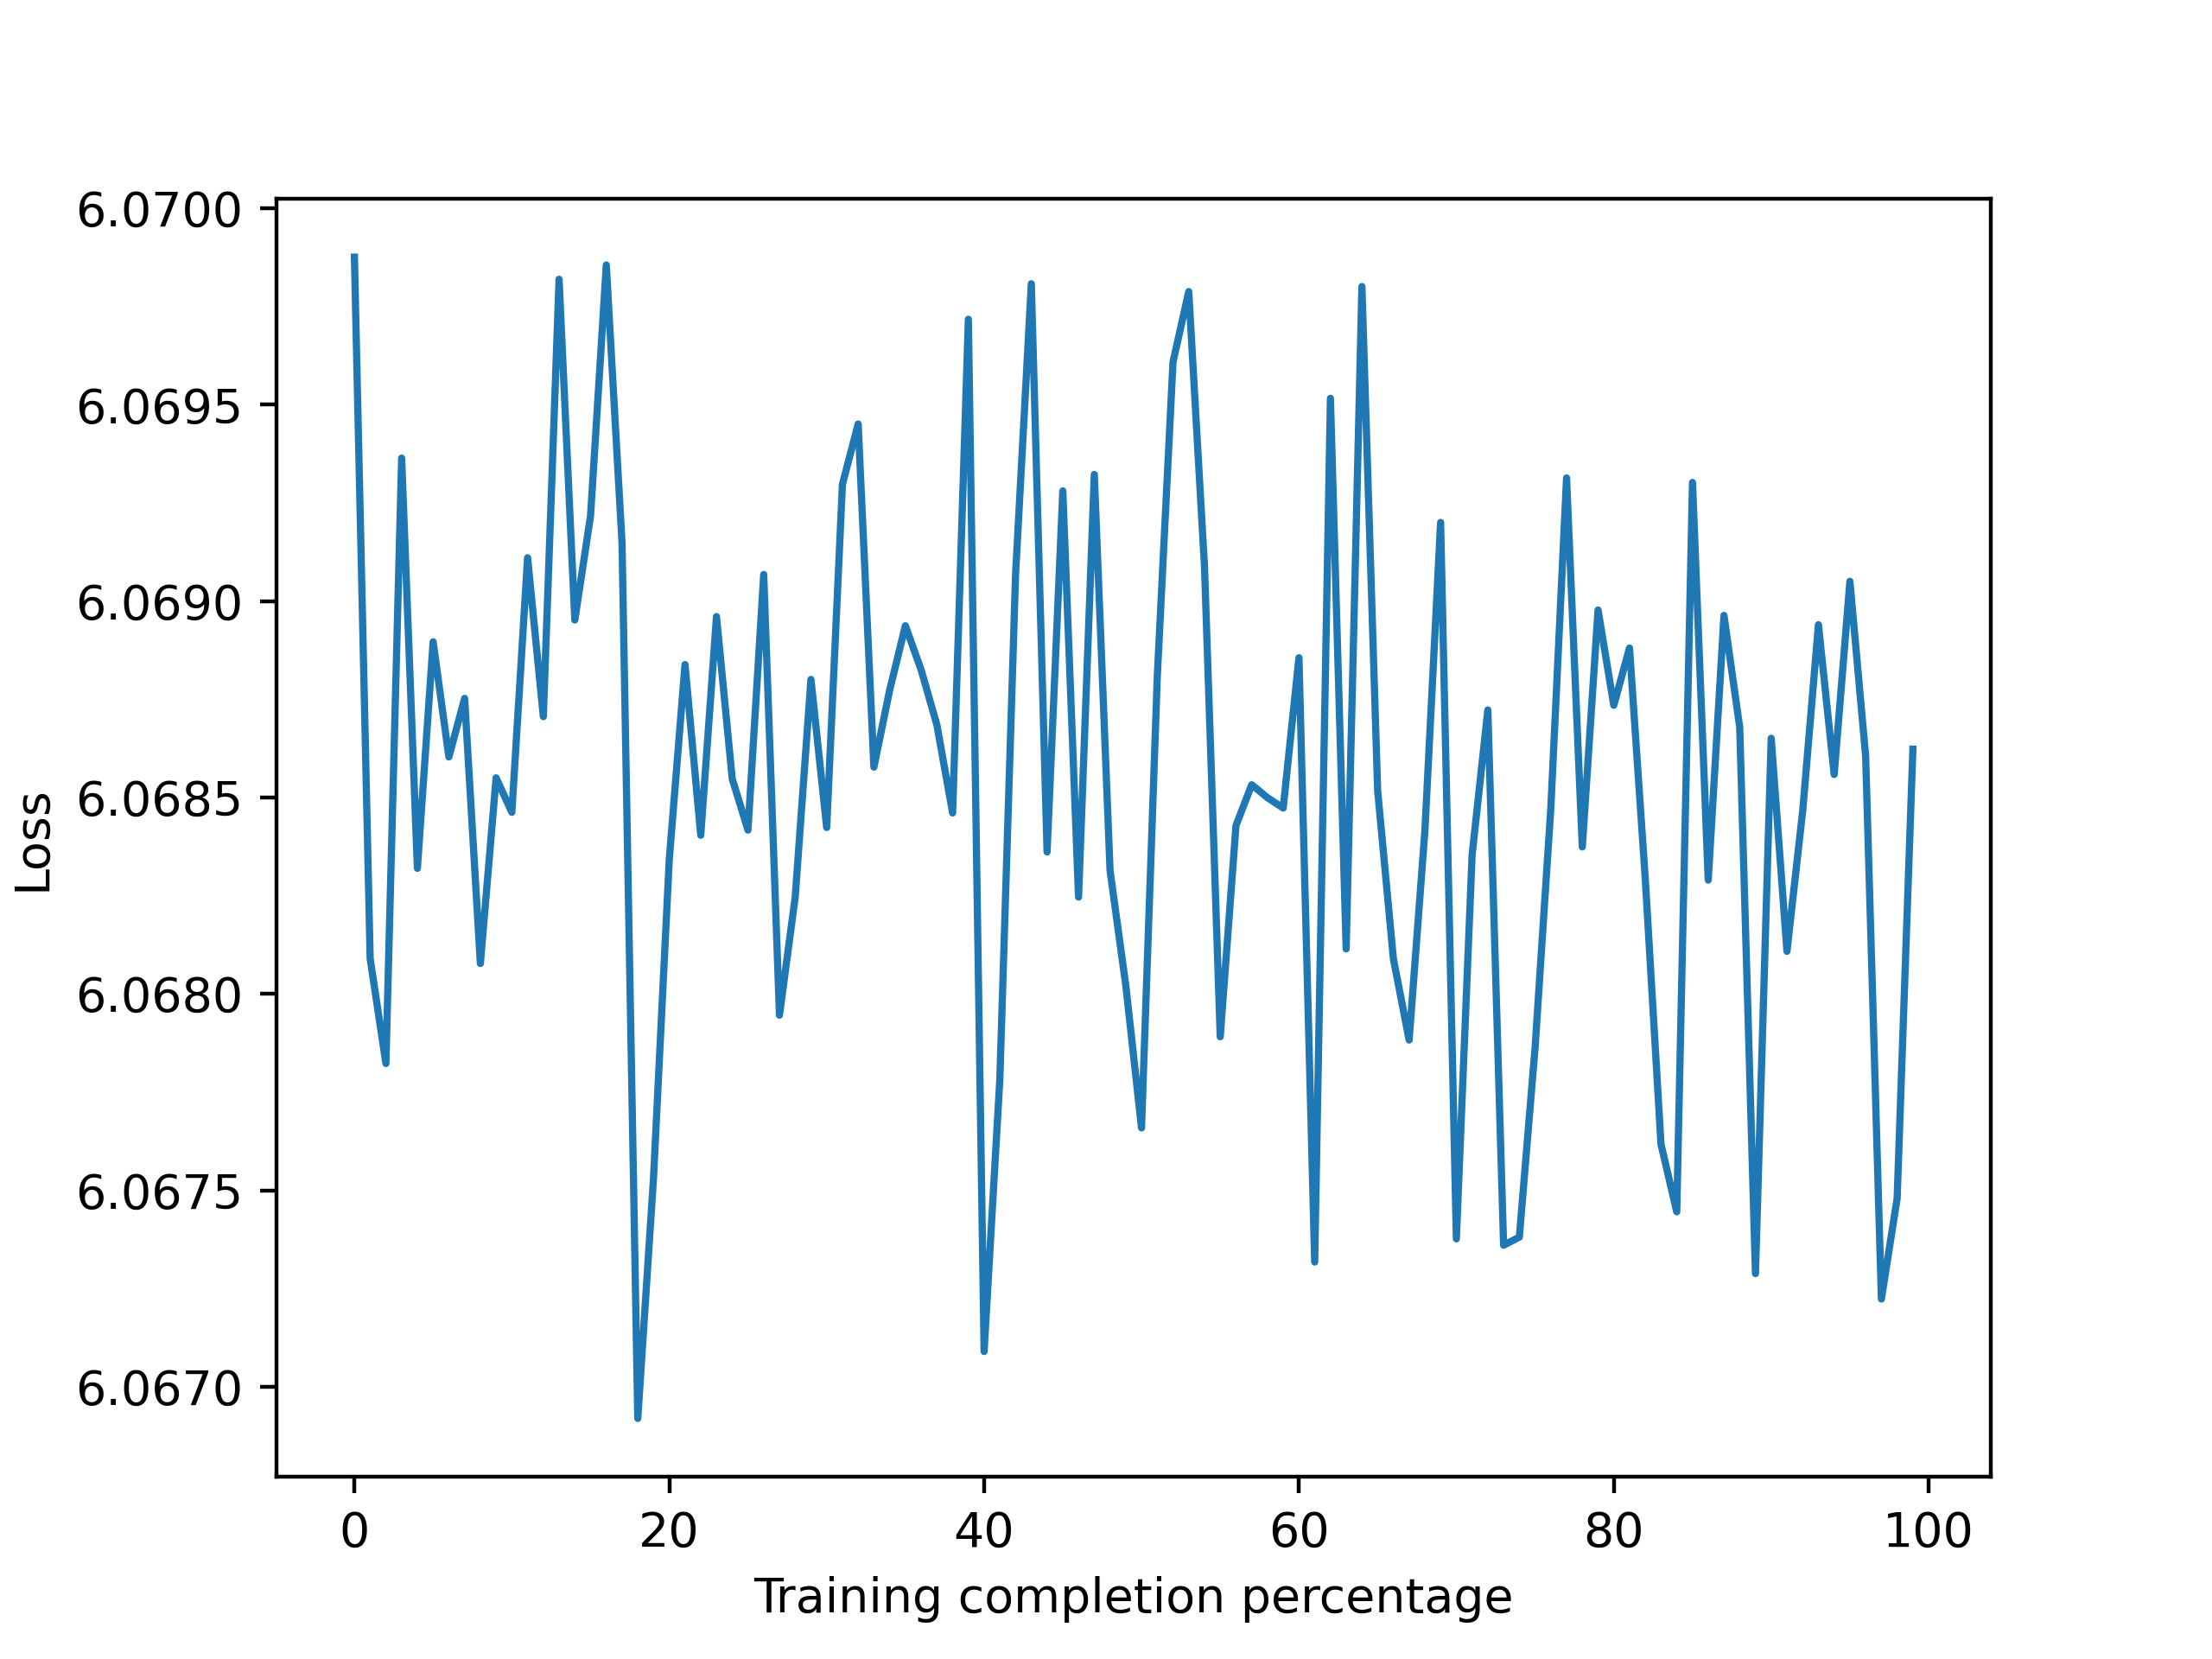
\includegraphics[scale=0.9]{loss_nograd.png}
        \caption{Loss without back propagation}
        \label{fig:nograd}
    \end{figure}
    
\end{enumerate}


\subsection{Training without updating the model parameters}
In this experiment, the \textbf{loss.backward()} method calculated the gradients. However, the model parameters were not updated by commenting the line number 16 and 17 from code listing \ref{code:train_function}. Notice in the figure \ref{fig:nograd} and figure \ref{fig:womp}, the loss is not reaching zero towards the end of the training. Indicating that in both the cases the model has not learned the product name patterns for the classification task.

\begin{figure}[H]
    \centering    
    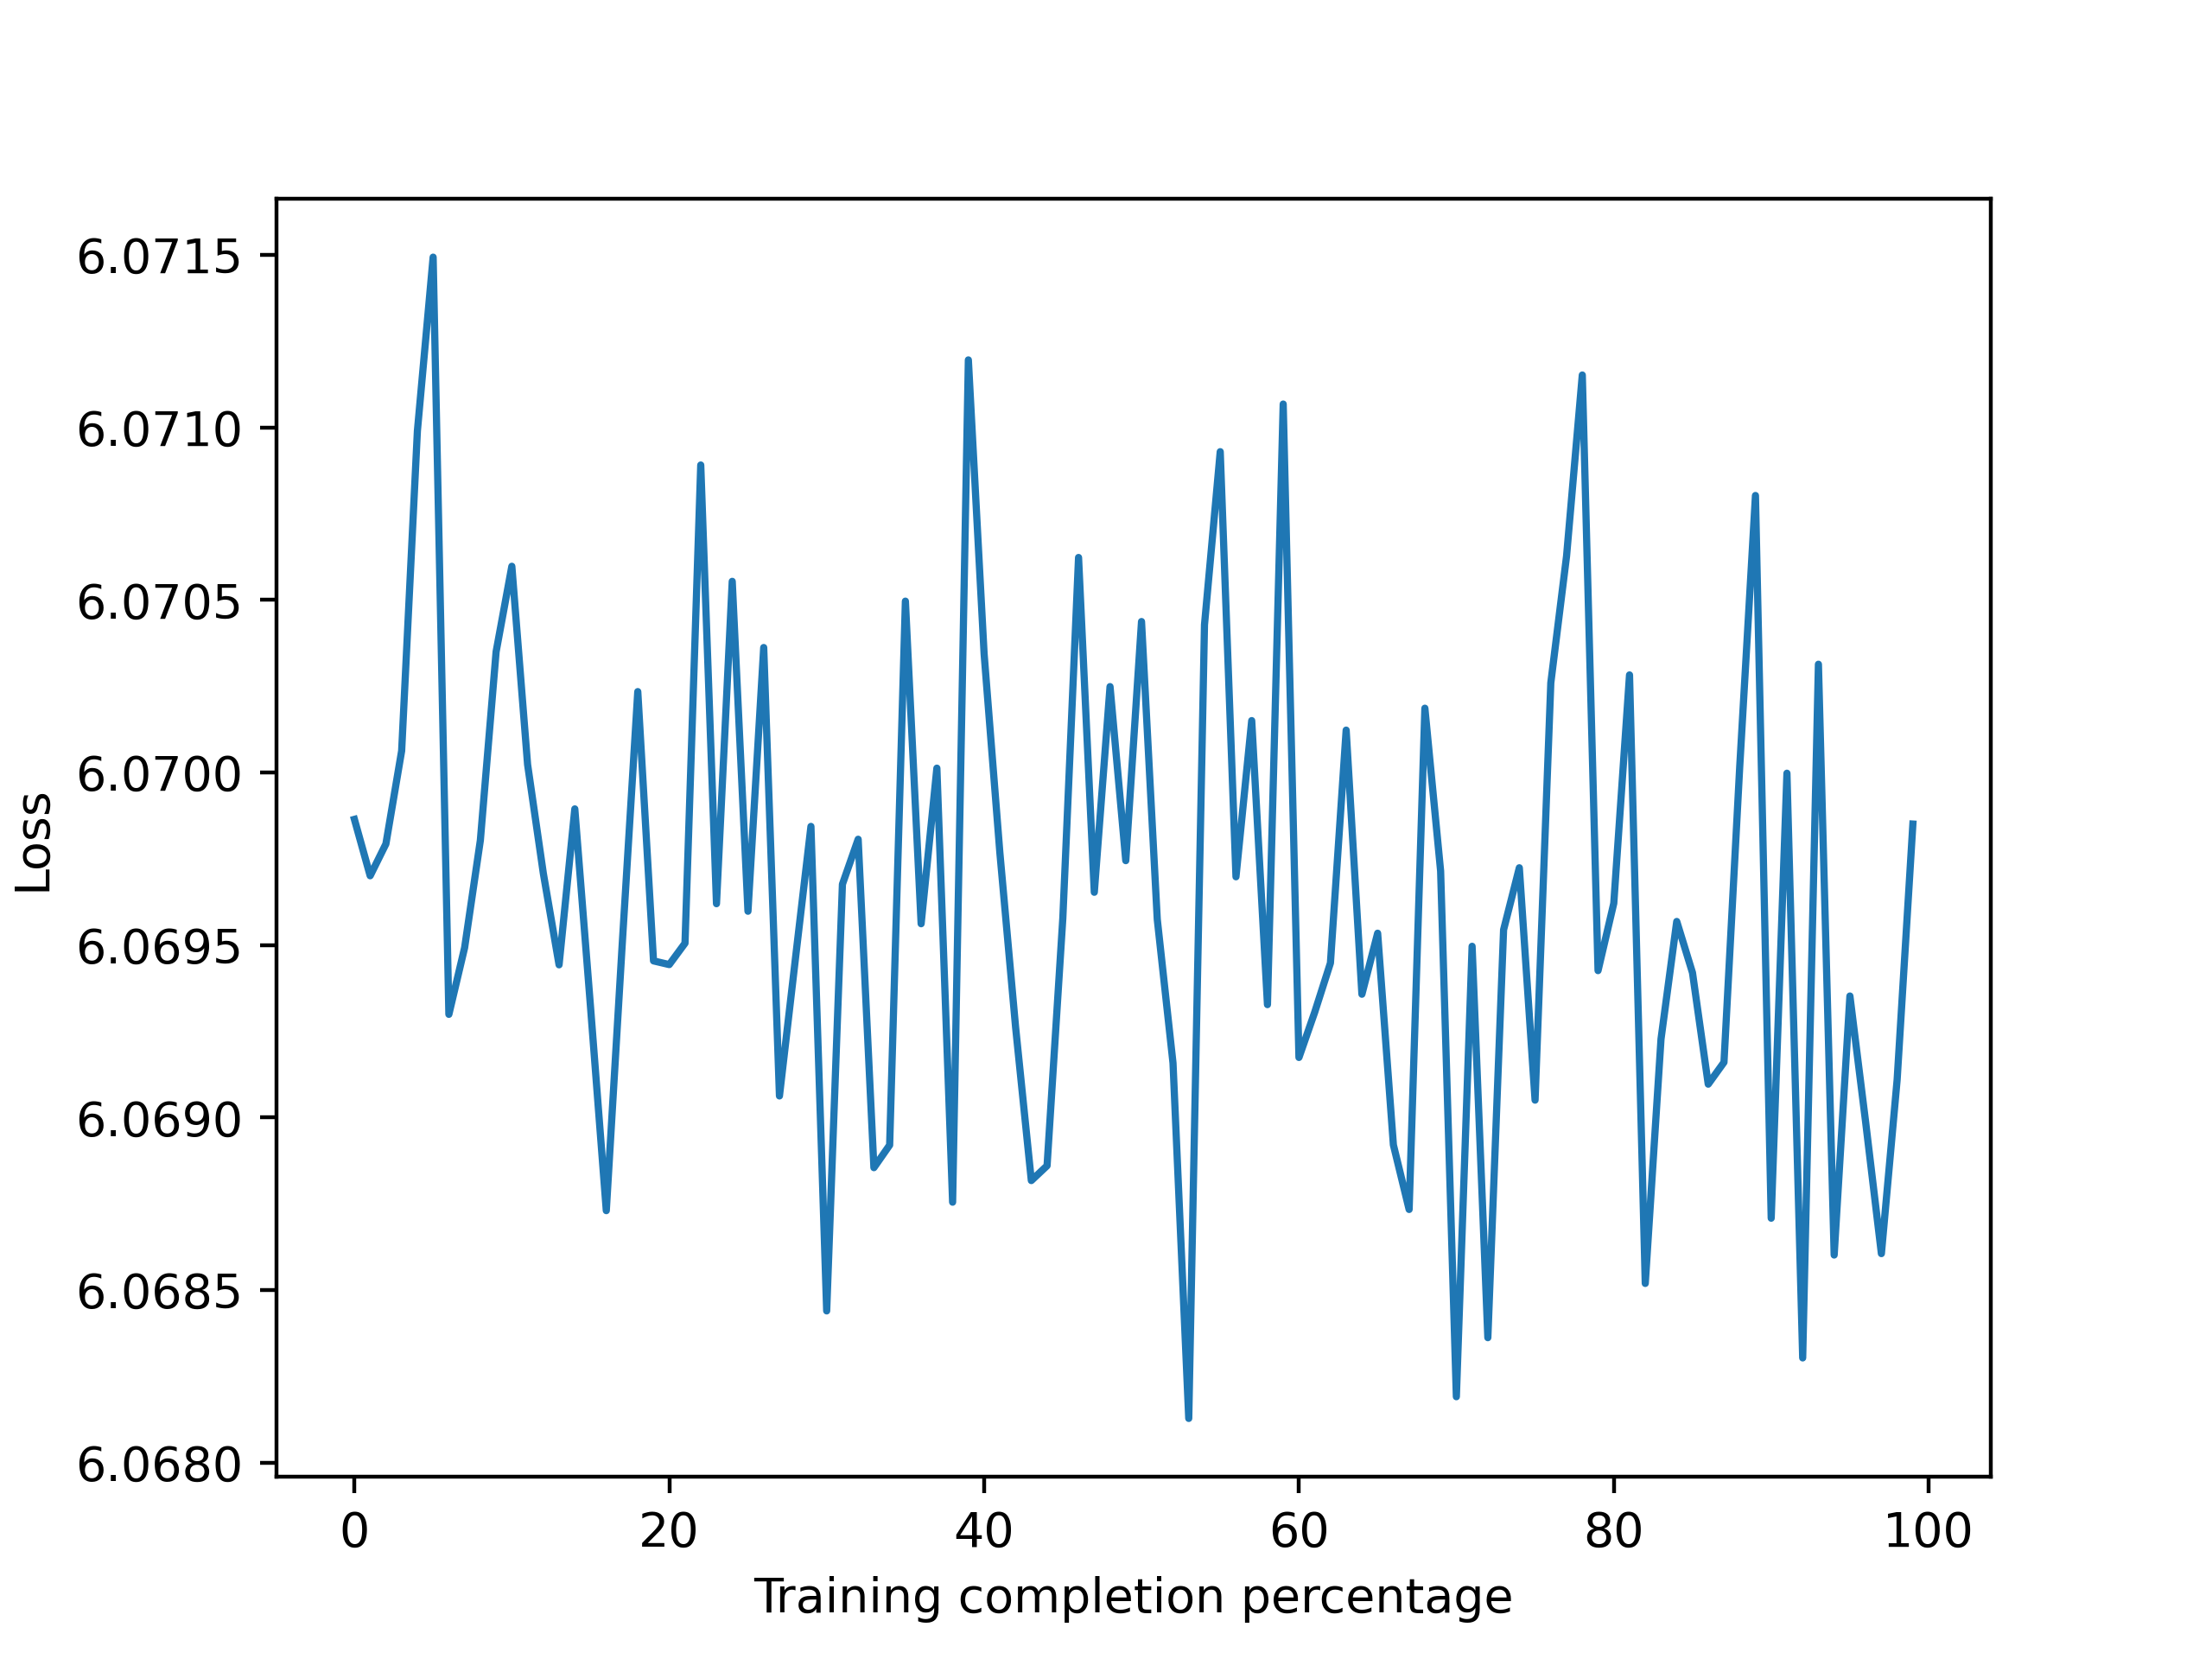
\includegraphics[scale=0.9]{loss_womp.png}
    \caption{Loss without updating the model parameters}
    \label{fig:womp}
\end{figure}

\subsection{Training with manually updating the model parameters} \label{sec:tmump}

The code listing \ref{code:mump} iterates through the parameters and updates their value based on the gradients computed during back propagation. 

\begin{lstlisting}[language=Python,caption={Manual gradient updation}, label={code:mump}]
    # Add parameters' gradients to their values, multiplied by learning rate
        for p in self.rnn.parameters():
            p.data.add_(p.grad.data, alpha=-self.learning_rate)
\end{lstlisting}

In code \ref{code:mump}, the parameter ``p.data'' is a tensor. The method  ``add\_()'' multiplies the argument and then add the product value to the tensor data ``p.data''. In this case, the negative value of ``learning\_rate'' is multiplied with the parameter gradient data and then the value is added to the ``p.data'' attribute.

\begin{figure}[H]
    \centering    
    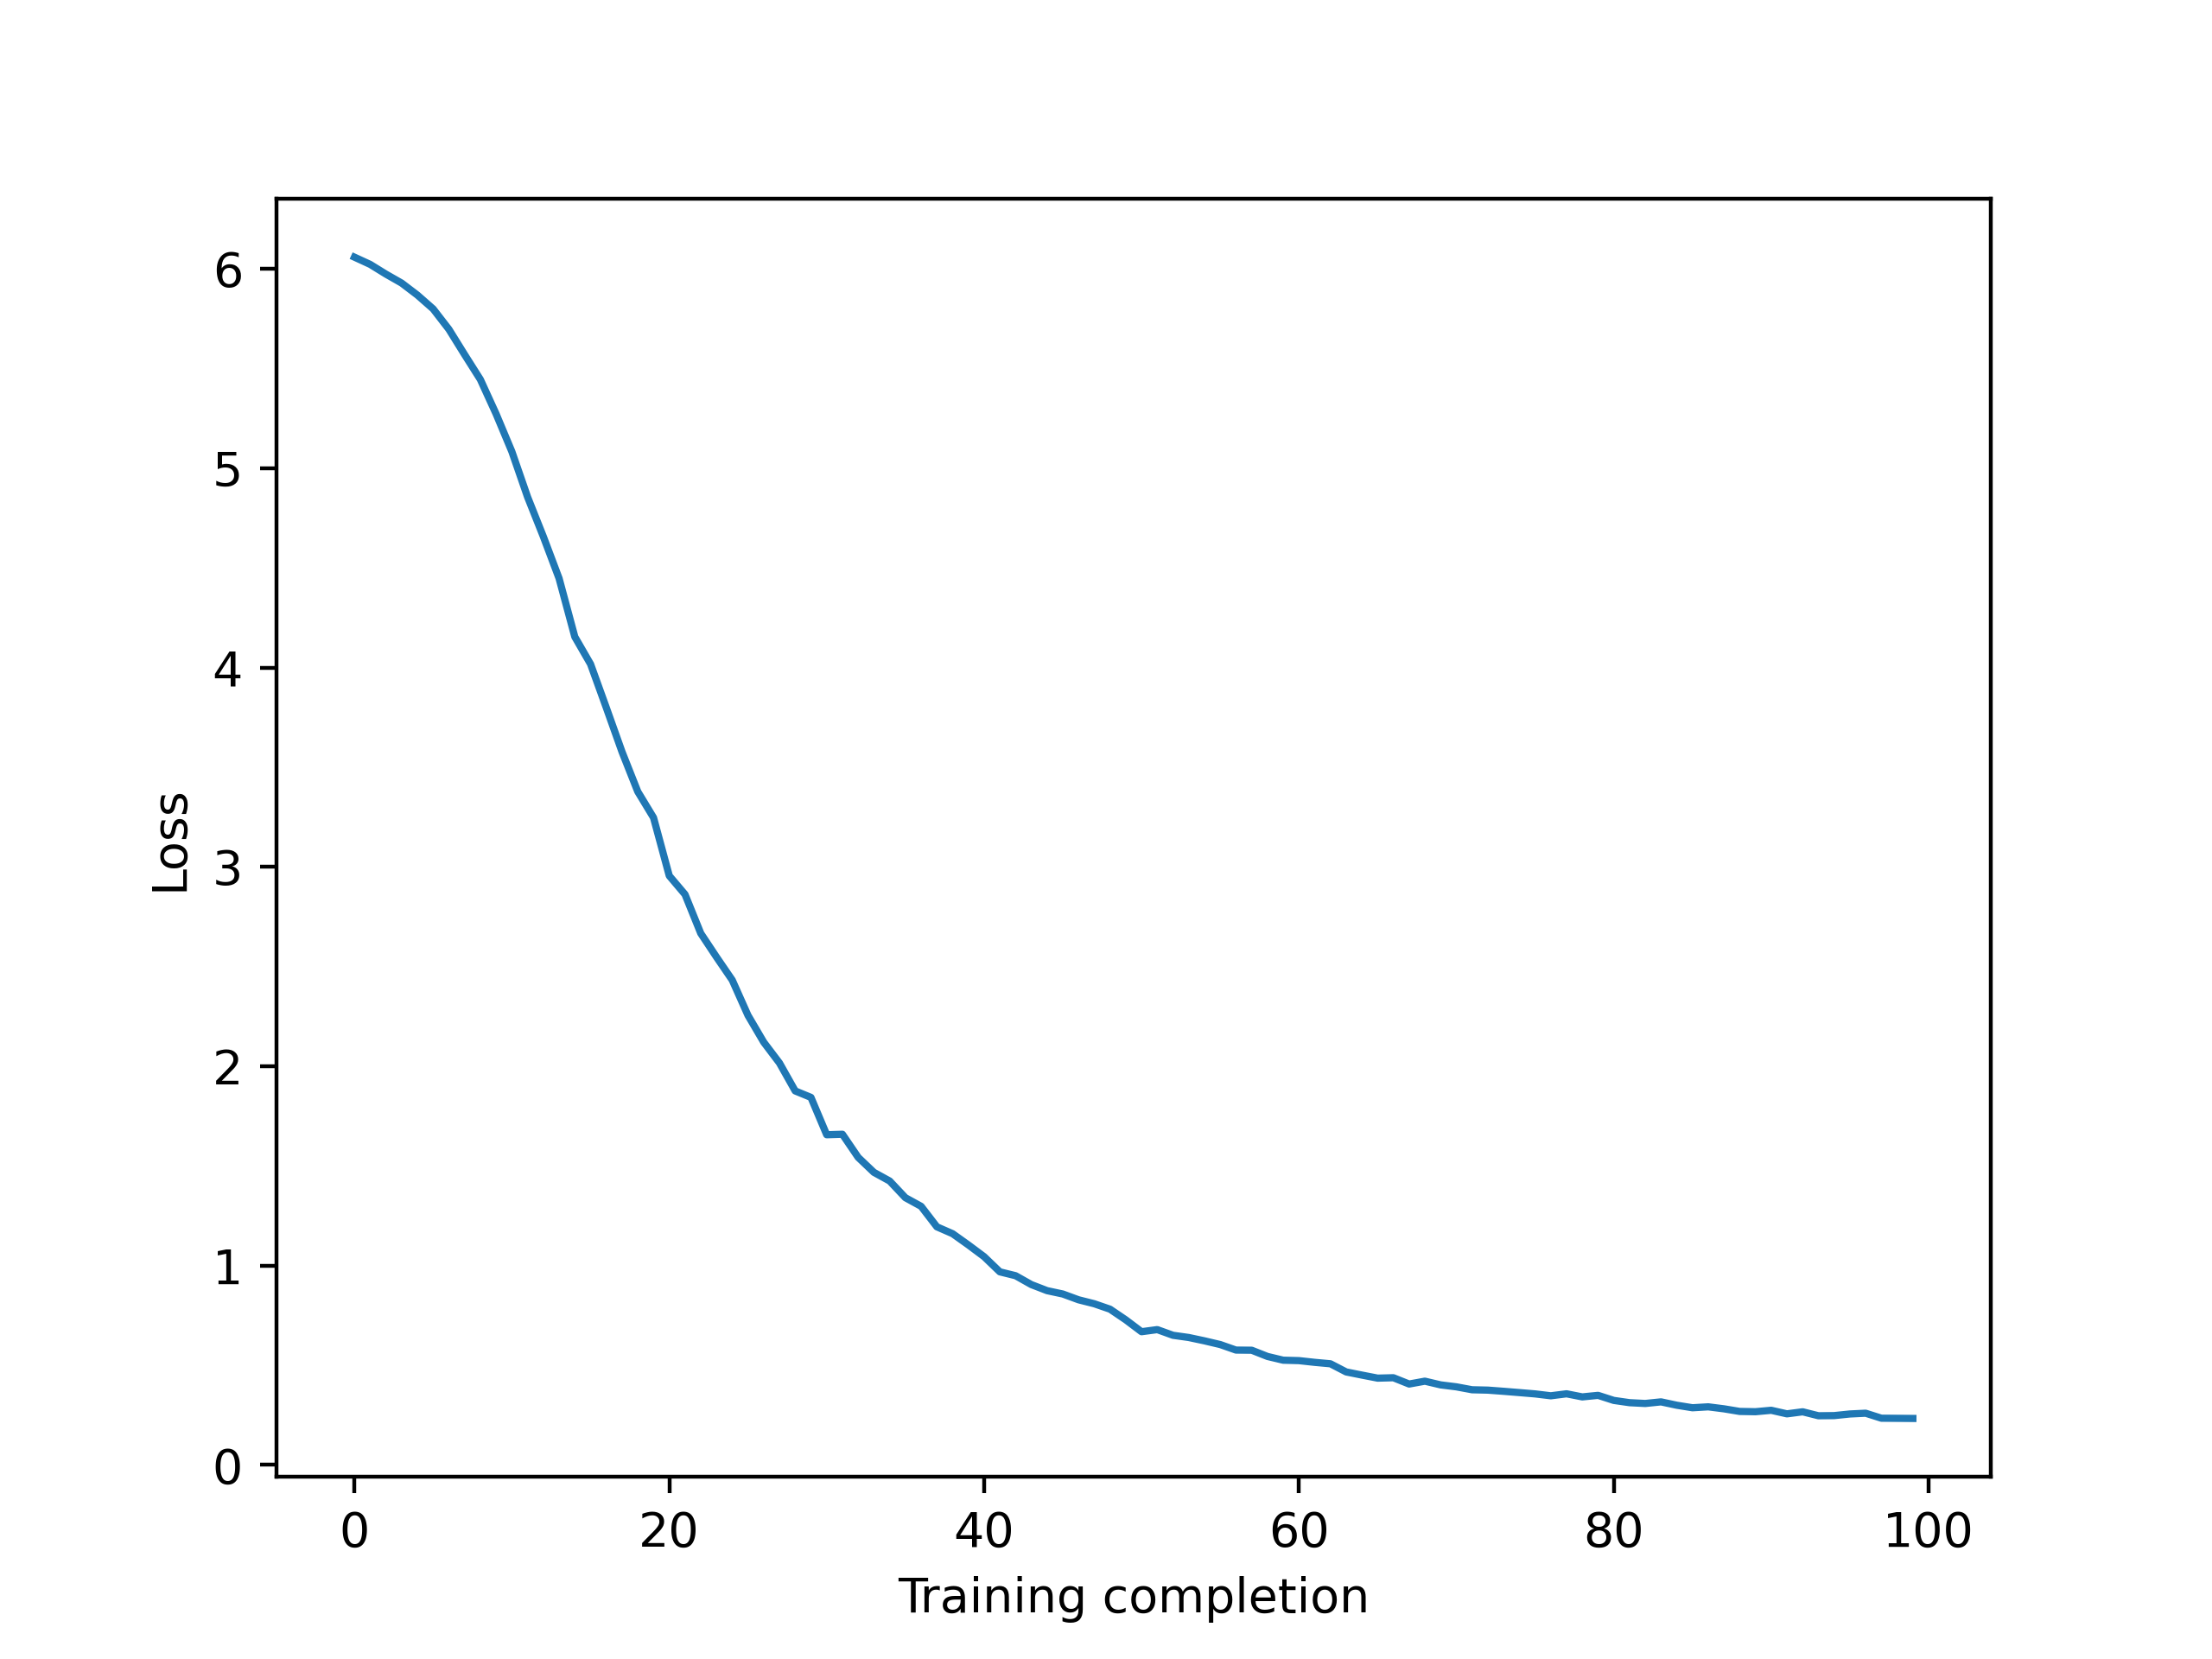
\includegraphics[scale=0.9]{loss_wmp.png}
    \caption{Loss with manually updating the model parameters with learning rate}
    \label{fig:wmp}
\end{figure}


\subsection{Updating the hidden number of units}

The model is described as a \acl{DAG} describing how functions are composed together. Consider having three functions $f(x) = f_3(f_2(f_1(x)))$ connected in a chain. $f_1$ is the first layer of the network, $f_2$ the second and so on. In the example of a classifier, $y=f_*(x)$ maps an input $ x $ to a category $ y $. The final layer of the network is called the output layer. The training data specifies what the output layer must do at each point $x$, that is to produce a value close to $y$. As the training data does not show the desired output for other layers, they are called \textbf{hidden layers}  \parencite[Chapter 3]{Goodfellow-et-al-2016}.  \parencite{zhang2021dive} describes the concept of \textbf{hidden state} which are inputs at step $t$ can only be computed with previous input at step $ t-1 $. \acf{RNN} are neural network with hidden states.

\subsubsection{Model with only one hidden state}
In this experiment, only one hidden state has been assigned to the \acs{RNN} network. As illustrated in figure \ref{fig:unihidden}, the loss reduces gradually. However, the model is yet under fit for the classification task. The loss not reaching zero towards the end of the training indicates that the model has not learned anything significant.

\begin{figure}[H]
    \centering    
    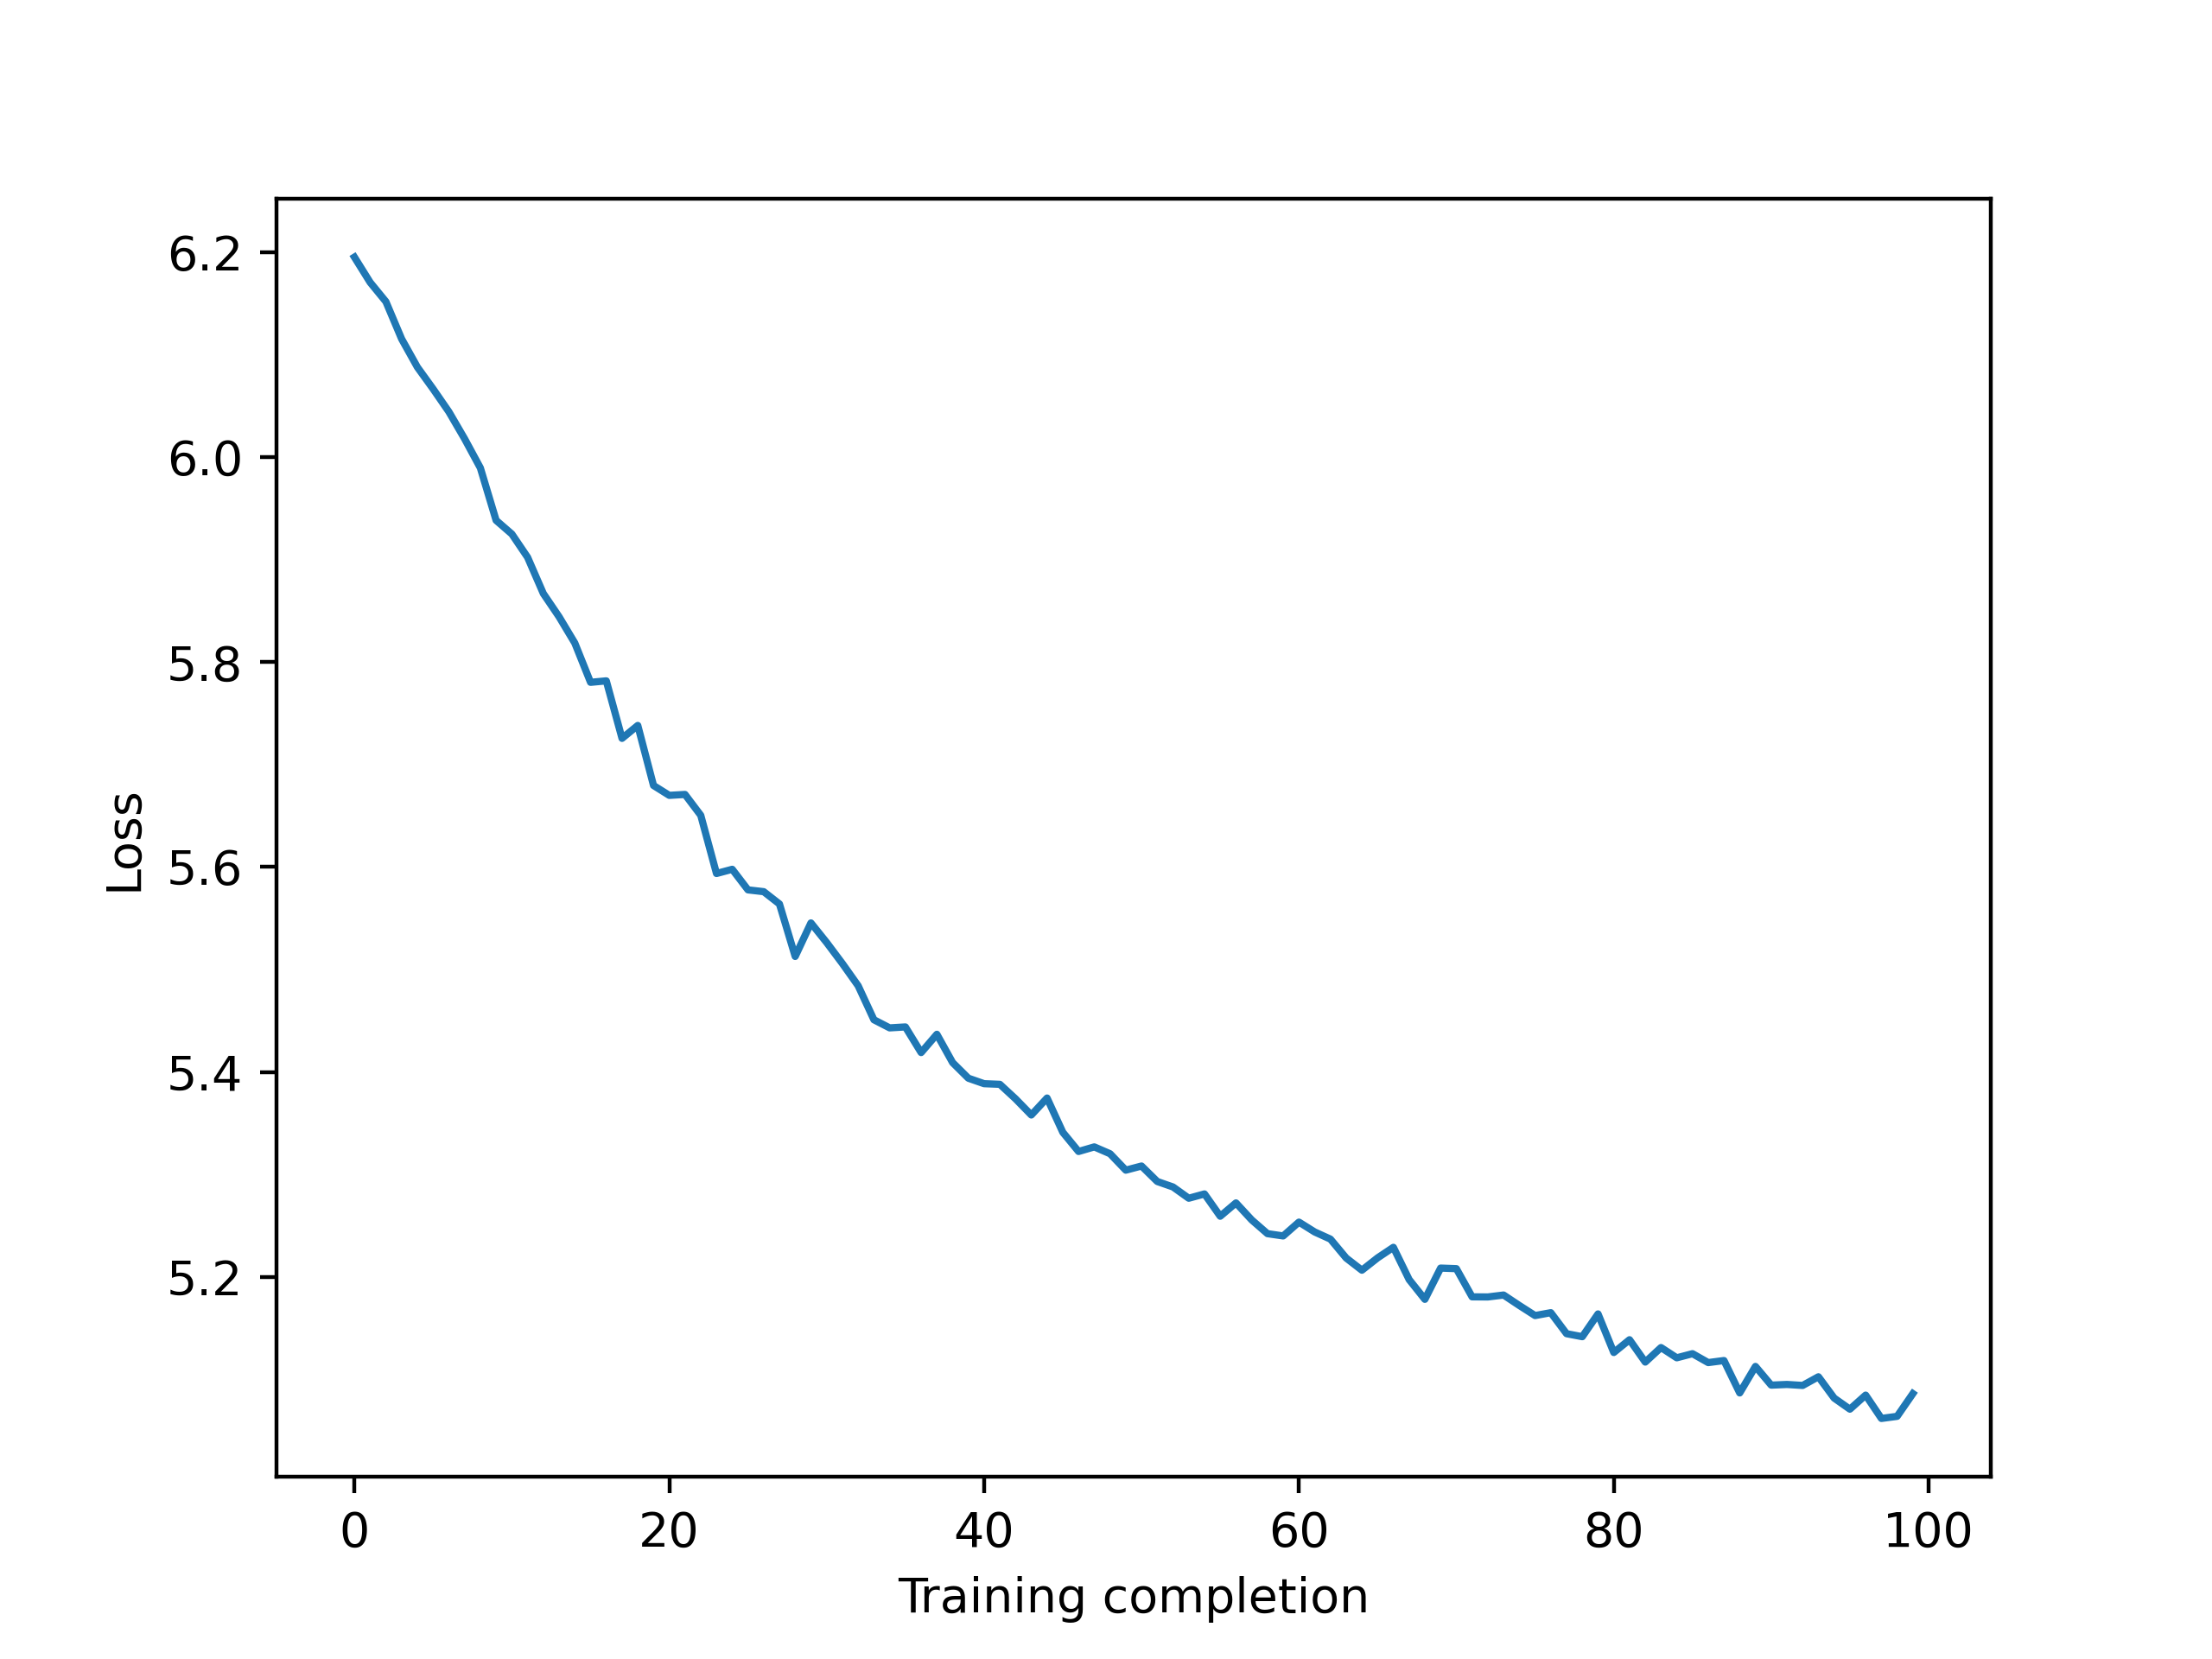
\includegraphics[scale=0.9]{loss_1hidden.png}
    \caption{Model with only one hidden state}
    \label{fig:unihidden}
\end{figure}

\subsubsection{Model with only 10 hidden state}
Increasing the number of hidden state to 10 units gave the desired result.  As seen in figure \ref{fig:10hidden}, the loss has reached near zero by end of the training. This model is able to predict the category based on the pattern of name.
\begin{figure}[H]
    \centering    
    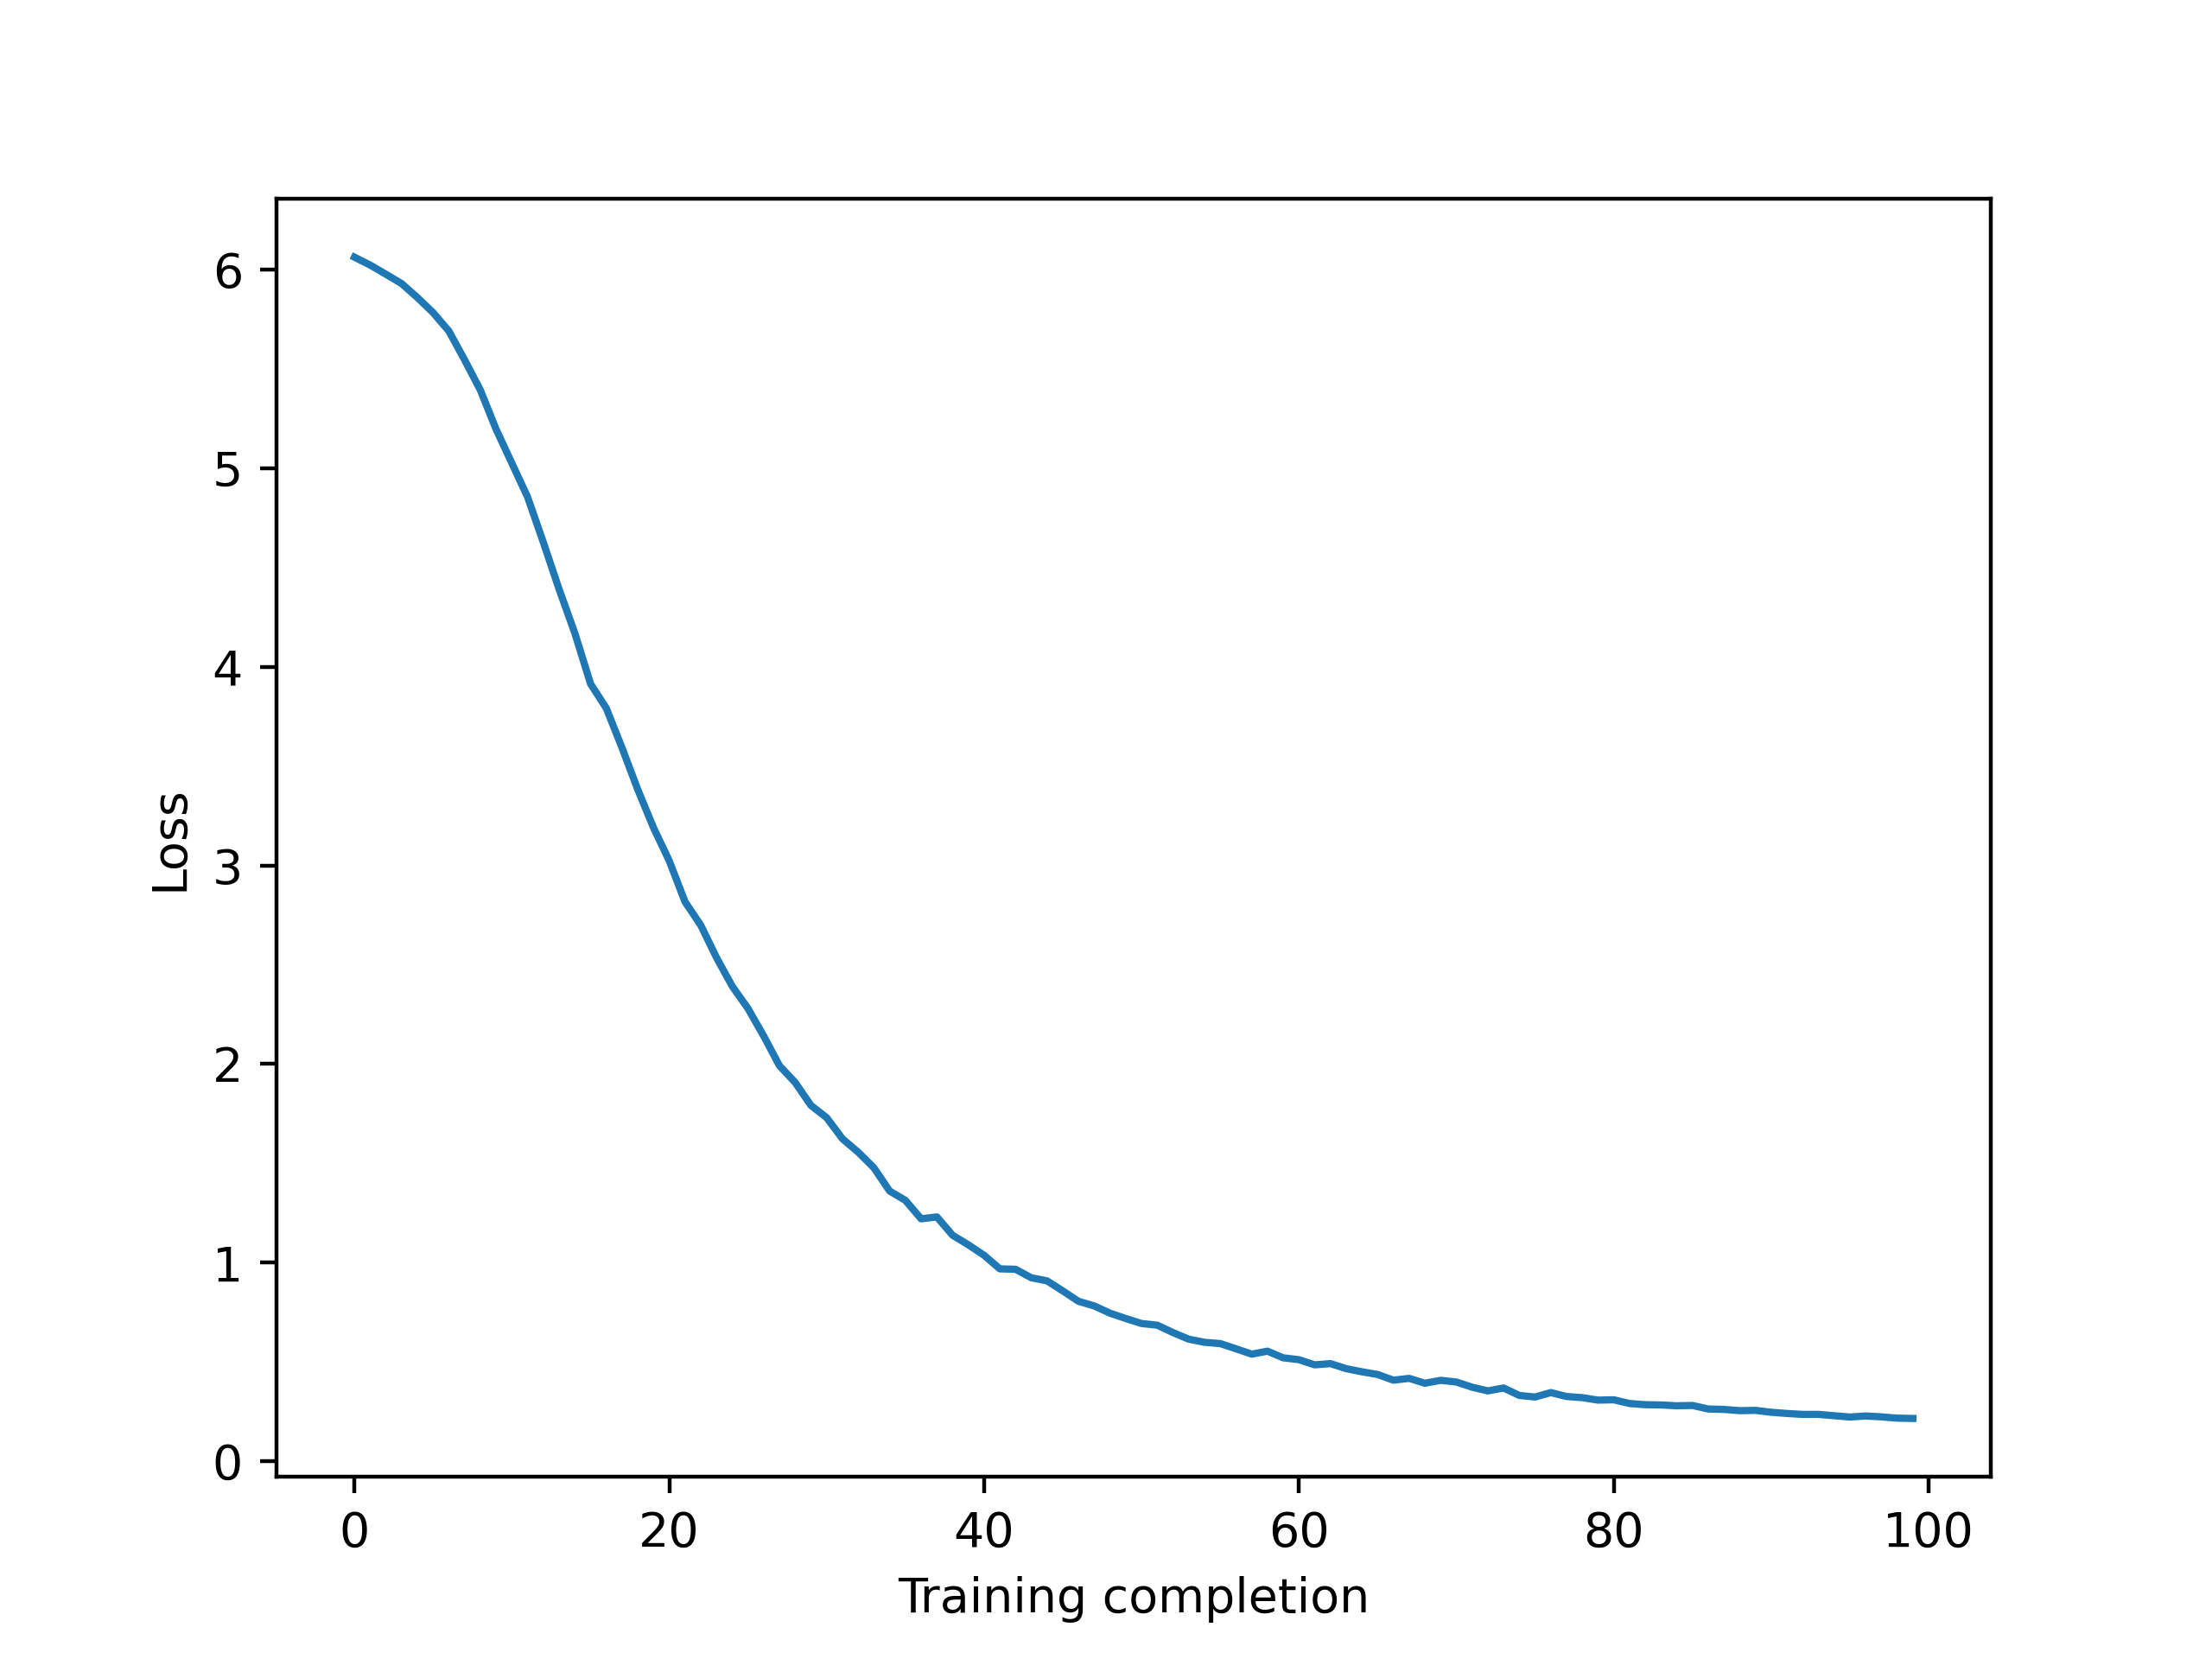
\includegraphics[scale=0.9]{loss_10h.png}
    \caption{Model with only 10 hidden state}
    \label{fig:10hidden}
\end{figure}

\subsection{Gradient decent step adjustment}

As stated in section \ref{sec:backward}, the method \textbf{loss.backward()} computes the gradients by applying chain rule of calculus for each function $f(x)$. The derivative of this function is denoted as $f'(x)$ \\ or as $\frac{dy}{dx}$. $f(x)$ can be reduced by moving $x$ in small with steps opposite sign of derivative is called gradient decent \parencite{cauchy}.  \parencite[section 4.3]{Goodfellow-et-al-2016} presents an equation \ref{eq:update_rule}.

\begin{align}
    x_i = x_i - \epsilon \frac{\partial}{\partial x_i} f(x) \label{eq:update_rule}
\end{align}

\begin{itemize}
    \item \( x_i \): The \(i\)th parameter of the model (weight or coefficient).
    \item \( \epsilon \): The learning rate, a positive scalar which determines the size of the step.
    \item \( f(x) \): The cost or loss function trying to minimize.
    \item \( \frac{\partial}{\partial x_i} f(x)\): The partial derivative  measures how \( f \) changes as only the variable \( x_i \) increases at point  \( x \).
\end{itemize}


In section \ref{sec:tmump}, refer to the code listing \ref{code:mump}, based on the equation \ref{eq:update_rule} we conclude that the variable \textit{p.grad.data} represents the partial derivative \( \frac{\partial}{\partial x_i} f(x) \) and the negative value of variable \textit{self.learninig\_rate} is included to subtract product of  variable \textit{p.grad.data} and variable \\ \textit{self.learninig\_rate} with variable \textit{p.data}. The same result can be achived by using pytorch's  \textit{subtract\_} method without negating the value of \textit{self.learninig\_rate}.

\begin{lstlisting}[language=Python,caption={Manual gradient updation with substract\_}, label={code:mumps}]
    # Add parameters' gradients to their values, multiplied by learning rate
        for p in self.rnn.parameters():
            p.data.subtract_(p.grad.data, alpha=self.learning_rate)
\end{lstlisting}

\section{\acf{CLR}}

Learning rate is an important parameter to tune the training of deep neural network. \parencite{Smith.03062015} describes a new method to set the learning rate called \acf{CLR}. In this method the learning rate in the training cyclically vary between the reasonable boundaries of the learning rate instead of having a fixed learning rate.

The steps involved in training a model with \acs{CLR} are as follows :

\begin{enumerate}
    \item Define the Learning rate range or reasonable boundary value: \\
    In this step, by linearly increasing the learning rate during training can specify the learning rate range in which an optimal accuracy is obtained. The lower point of range can be referred as $base\_lr$ and higher point as $max\_lr$.
    \item Training the model by gradually decreasing the learning rate to $base\_lr$ and again increasing the learning rate to $max\_lr$ over an interval of a constant step size.
\end{enumerate}


\subsection{Experimentation and analysis to determine learning rate range}

\begin{enumerate}
    \item Experiment by setting $base\_lr$ and $max\_lr$  manually : \\
    In this experiment, the learning rate range is set manually to very low and high values. Numpy np.linspace() \parencite{harris2020array} returns the evenly spaced numbers between the  $base\_lr$ and $max\_lr$ over a specified interval.

    The result of training process the model with $base\_lr =1 \times 10^{-11}$ and $max\_lr=0.9$.\\
    In figure \ref{fig:Loss value} notice that at 32 \% of training completion with learning rate $\approx$ 0.2 the loss started to explode. Hence, we conclude that the  $max\_lr < 0.2$

    \begin{figure}[H]
        \centering    
        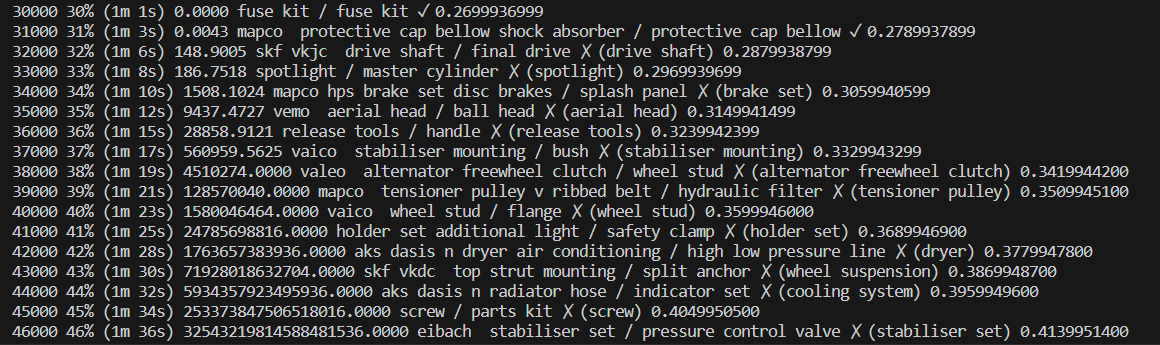
\includegraphics[scale=0.7]{loss_nan.png}
        \caption{Result: Loss value returning nan}
        \label{fig:Loss value}
    \end{figure}


    \item In the next experiment, we set the $max\_lr = 0.2$. \\
    The classification model successfully completed the training and was able to predict the category.
    \begin{figure}[H]
        \centering    
        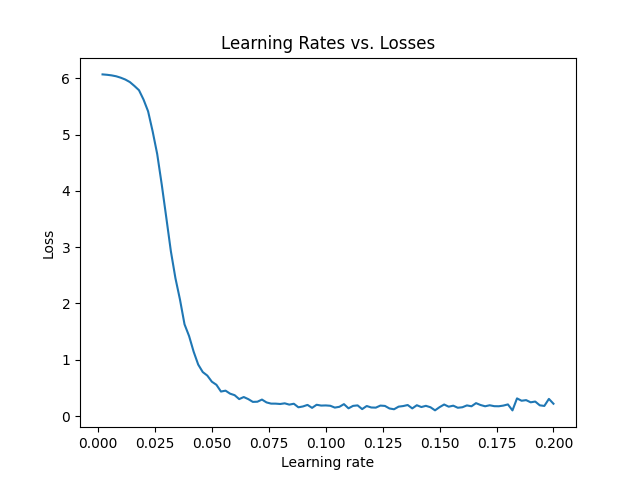
\includegraphics[scale=0.9]{loss_lr_02.png}
        \caption{Loss vs Learning rate; where $max\_lr = 0.2$}
        \label{fig:Loss value at 0.2}
    \end{figure}
    
    As illustrated in figure \ref{fig:Loss value at 0.2}, in the graph plotted of Loss Vs Learning rate. The model started to learn at learning rate $\epsilon = 0.04$ onwards. We will further reduce the $max\_lr$.

    \item In the next experiment, we set the $max\_lr = 0.04$. \\
    Notice in figure \ref{fig:Loss value at 0.04}, there is a plateau until $\epsilon = 0.010$. After which there is a descent until $\epsilon = 0.015$
    \begin{figure}[H]
        \centering    
        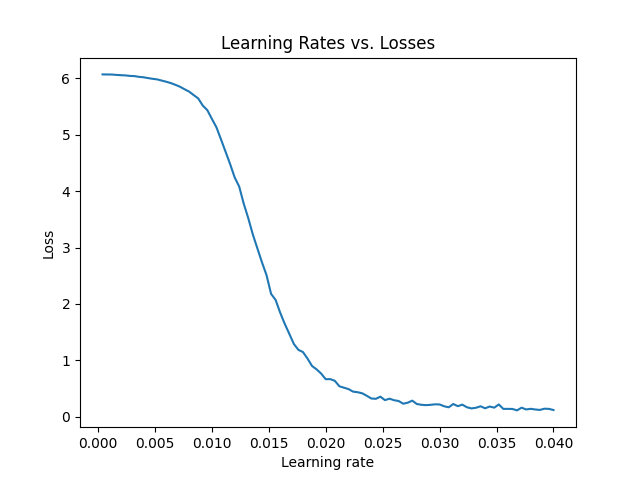
\includegraphics[scale=0.9]{loss_004.png}
        \caption{Loss vs Learning rate; where $max\_lr = 0.04$}
        \label{fig:Loss value at 0.04}
    \end{figure}

    \item In the next experiment, we set the $max\_lr = 0.015$. \\
    Notice in figure \ref{fig:Loss value at 0.015}, the loss had not neared zero and the model fails to predict the classification. 
    \begin{figure}[H]
        \centering    
        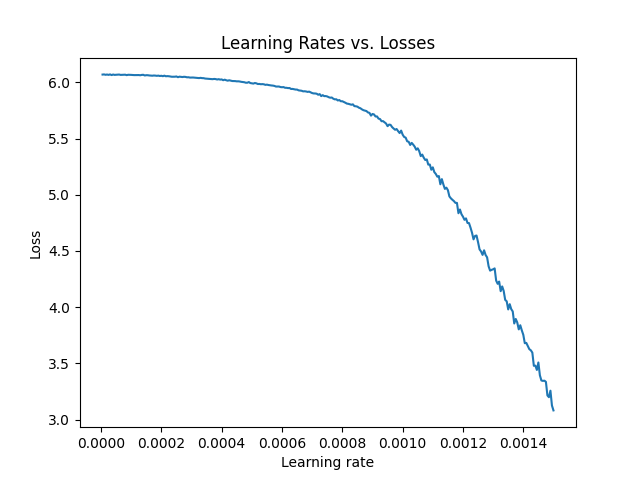
\includegraphics[scale=0.9]{loss_0015.png}
        \caption{Loss vs Learning rate; where $max\_lr = 0.015$}
        \label{fig:Loss value at 0.015}
    \end{figure}

    \item From the earlier mentioned experimentation with $max\_lr$,  the loss classification model is nearing zero by the end the training  when  $max\_lr > 0.015$ 
    Figure \ref{fig:Loss value at 0.02} illustrates the loss reaching near zero when $max\_lr = 0.02$. The figure  \ref{fig:Loss value at 0.02}, there is a plateau until the $ \epsilon = 0.0075$. Indicating that the model did not learn until the learning rate $ \epsilon = 0.0075$.
    \begin{figure}[H]
        \centering    
        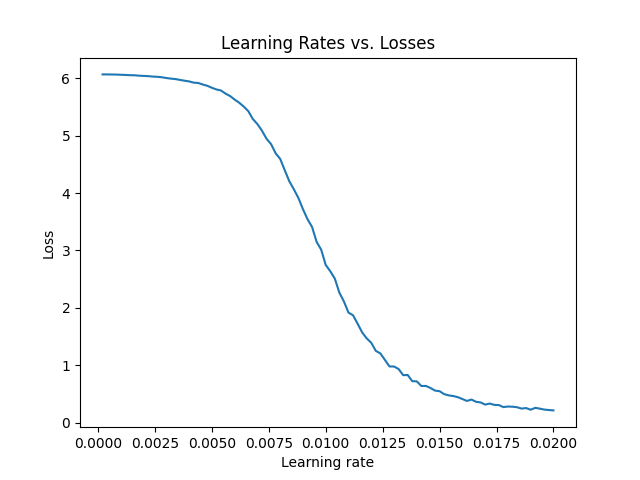
\includegraphics[scale=0.9]{loss_002.png}
        \caption{Loss vs Learning rate; where $max\_lr = 0.02$}
        \label{fig:Loss value at 0.02}
    \end{figure}

    \item Updating the $base_lr=0.0075$ and $max_lr=0.02$, resulted a steady slop in the loss vs learning rate.  
    Figure \ref{fig:Loss value at 0.0075} illustrates the loss reaching near zero when $max\_lr = 0.02$ and $base_lr=0.0075$. The steady decent indicates the learning rate range is optimal.
    \begin{figure}[H]
        \centering    
        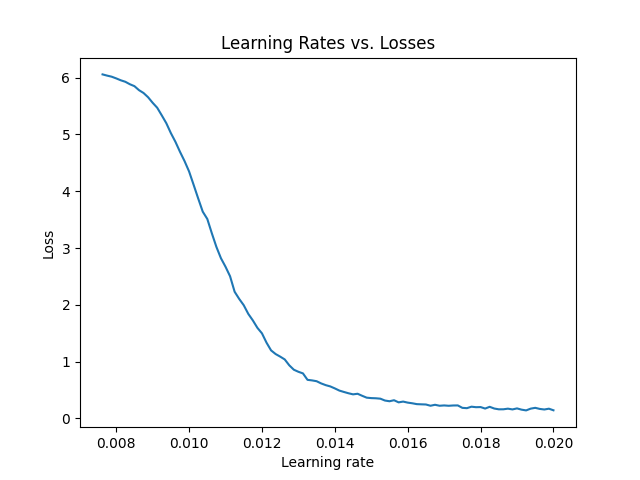
\includegraphics[scale=0.9]{loss_0075_002.png}
        \caption{Loss vs Learning rate; where $base\_lr = 0.0075$ and $max\_lr = 0.02$ }
        \label{fig:Loss value at 0.0075}
    \end{figure}
    

\end{enumerate}

\section{Triangular learning rate}

\parencite{Smith.03062015} introduced the concept of letting the learning rate vary within the range of minimum and maximum boundaries of learning rate known as learning rate range. In this method the learning rate linearly increases until step size $ t $ and then linearly decreases. 


How triangular learning rate works?

\begin{enumerate}
    \item \textbf{Initialize}: The step size $ t $, minimum bound or base learning rate $ base\_lr$ and maximum bound or the max learning rate  $max\_lr$ are initialized. These hyperparameters are tuned based on the architecture of the model. In this experiment, the values set are  $ base\_lr=0.0075 ; max\_lr=0.02; t=10000$.
    \item  \textbf{Up}: During training, the learning rate is linearly increased from $ base\_lr$ to $max\_lr$ over a certain number of step size $ t $.
    \item \textbf{Down}: During training, the learning rate is linearly decreased from $max\_lr$ to $base\_lr$.
\end{enumerate}

\begin{figure}[H]
    \centering    
    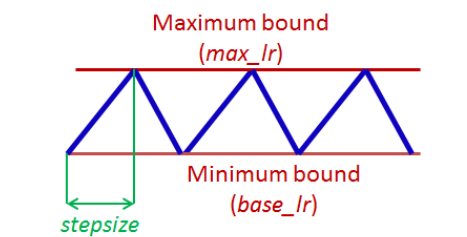
\includegraphics[scale=0.9]{triangular learning rate.png}
    \caption{Triangular learning rate policy.  \parencite{Smith.03062015}
    }
    \label{fig:trl}
\end{figure}
 In figure \ref{fig:trl}, the blue lines represent learning rate values changing between the bounds. The input parameter stepsize is the number of iterations in half a cycle \parencite{Smith.03062015}.

\chapter{Building a Knowledge graph} \label{sec:building-kg}

Graph-based knowledge representation has been researched for decades.
A \acf{kg} acquires and integrates information into an ontology and applies a reasoner to derive new knowledge \parencite{LisaEhrlinger}.
The knowledge base is a dataset with formal semantics that can contain different kinds of knowledge, for example, rules, facts, axioms, definitions, statements, and primitives \parencite{Davies.2008cop.2006}.

\begin{figure}[h!]
    \centering
    \includesvg[scale=0.5]{Thesis_kg.svg}
    \caption{\acl{kg} architecture}
    \label{fig:kg}
    \parencite[Chapter 4]{LisaEhrlinger}
\end{figure}

Figure \ref{fig:kg} illustrates the procsssing of plain text from various sources such as  Wikipedia API, PDF into a graph. This abstract architecture represented by \Citeauthor{LisaEhrlinger} of a \acl{kg} portraits the asumption that a \acl{kg} is more than a \acf{kb}. \acl{kg} is a combination of \acl{kb} and \acf{qe}. 

\Iac{qe} is a set of graph of possible questions that could be formed in reference to \iac{kb}. \acf{qg} for comprehensive reading is a challenging task. There are datasets available for  \acs{qg}, one of it is Stanford Question Answering Dataset v1.0 (SQuAD) consisting of questions posed by crowdworkers on a set of Wikipedia articles \parencite{PranavRajpurkar.}. The limitation with such a data set is that these do not contain unanserable questions. Building a machine learning model when no answer is supported was out of scope of SQuAD objective \parencite{LupeHernandez}.  Study on automatic question generation from an attention-based sequence learning model for  \ac{qg} and investigate the effect of encoding sentence- vs. paragraph-level information \parencite{DuXinya.29042017}, reduces reliance on handcrafted rule based systems.

\clearpage

\section{Fetching text corpus}


One of the first things required for \acf*{nlp} tasks is a creating a text corpus.
In linguistics and \acs{nlp}, corpus refers to a collection of texts. One of the objective of this paper is to web crawl and extract data related to "Motor Oil". Our intention is to fetch the unstructred text corpus specifically related to "Motor Oil" and to create a graph-based knowledge. 

Wikipedia\footnote{https://www.wikipedia.org/} is primarily an encyclopedia with the additional benefit of heavy linking between articles and without the size constraints of paper articles \parencite{TorstenZesch}. Wikipedia API \footnote{https://pypi.org/project/Wikipedia-API/}

\section{spaCy - Dependency Parsing} \label{dependencyparsing}

spaCy \parencite{spacy2} features neural models for parsing and entity recognition. These models can be trained for \acf{ner} , tagging and parsing. Its official page on usage\footnote {https://v2.spacy.io/usage/} provides in-depth code example for information extraction.

In figure \ref{fig:dp}, we see a complex sentence's dependency parsing. It has a \acf{nsubj}, connecting \acfp{pobj} with \acfp{adp} and no \acf{dobj}.

\begin{figure}[htp!]
    \centering    
    \includesvg[scale=0.16]{dependency-parser.svg}
    \caption{Navigating the parse tree and subtrees}
    \label{fig:dp}
\end{figure}

The \acs{nsubj} "oil", itself does not give a complete meaning. However, upon combining its dependency noun "Motor", which is "Motor oil"  gives us an understanding of the topic. Traversing from \acs{nsubj} to  \acfp{conj} provides us with three related compound nouns belonging to a similar group.

"Motor oil", "Engine Oil", "Engine Lubricant"

Traversing further right of the dependency tree we can extract the \acsp{pobj}.  An \acf{amod} "internal" is connecting compound noun "combustion engine".

\section{Knowledge graph with Networkx}

The directed graphs created with Networkx \parencite{hagberg2008exploring} is suitable for representing depedency parsing of a sentence mentioned in section \ref{dependencyparsing}. A knowledge base are represented as triples of \acf{SRO}. In which the subject and object are nodes or entities of a graph and relation are directed edges or links between the nodes.

\subsection{What to use as nodes n(x) and edges e(y)?}

In table \ref{table:1}, distigution of triples by  \acs{POS} tags is depicted. 
\begin{table}[h!]
\begin{center}
\begin{tabular}{>{$}l<{$} l}

triples   &   \acf{POS} tags   \\
\hline
n(subject)   &   \acs{nsubj} , \acs{pron}                          \\
n(object)  &   \acs{dobj}    , \acs{pobj}                     \\
e(relation)  &   \acs{adp}, verb
\end{tabular}
\end{center}
\caption{\acs{SRO} and \acs{POS} tags mappings}
\label{table:1}
\end{table}

\section{Summary}


In this chapter, using the dependency parsing of an unstructured sentence, building a knowledge graph is proposed.  The process involves textual information on a product from various sources pass through various methods such as dependency parsing, part of speech tagging, named entity relationship mapping. The processed text is created into a directed graph along with the question engine is called the knowledge graph.  

Further research has to be conducted on generating knowledge graph. As per \parencite{LisaEhrlinger}, there are limitations with knowledge graphs as comprehensive reading is a challenging task.
\chapter{Conclusion and Outlook}


\section{Answer to Research Questions}
\begin{enumerate}[label=\textbf{RQ\arabic*:}]
    \item What are the use cases in which natural language processing and machine learning model can be utilized in an E-Commerce industry?
    
    Machine learning model can generate well-defined product taxonomy. Author introduces a methodology for such a model in section \ref{sec:ideate}. A well-defined product taxonomy is the foundation for many use cases like the ones listed below:
        \begin{itemize}
        \item Product recommendation system.
        
        The machine learning model can classify and recommend products from the wide range of products to the customer based on the customer's transaction history. The transaction history containing product relevance feedback such as click ``clicks'', ``cart-adds'', ``orders'', ``revenue'' \parencite{KarmakerSantu.2017} are usable if the taxonomy is well-defined. 
        
        \item Search bar autocompletion.
        
        A lot of research has been conducted in the field of user experience in terms of product search. A facet in user interface is an extended drop down menu with filtered result set. \parencite{Tagliabue.26052020} proposes a real time personalized catalog generation by combining customer search logs and in-session data. 
        
        \item Customer conversational shopping.
            
        \Parencite{ChrisMessina} states that gradually traditional commerce will shift towards conversational commerce. An experience of shopping on the go or hands-free assistance could be trending. Major Ecommerce  industries offering voice assistance devices includes feature of buying products on voice command.  


        \item Building a knowledge graph based on the textual details of a product. Refer section \ref{sec:building-kg}
        \item Virtual customer support chatbot may leverage the knowledge graph to answer queries raised by customers.
    \end{itemize}
    
    \item For a product classification task, how to define product features as an input for machine learning model?
    
   Based on the level of product taxonomy the number of features may vary. Table \ref{table:feature_decription} lists some features are listed simply by prior knowledge of the product domain. However, section \ref{sec:feature-selection} describes various methods to reduce dimensionality.

    
    \item How does a machine learn pattern in product features for classification?
    

    \begin{enumerate}[label=\textbf{SRQ\arabic*:}]
        \item What are the mathematical equations behind the learning process?
    
        Author has dedicated Chapter \ref{ch:math-behid} for step by step illustration of learning process. Author begins the chapter with basic mathematical representation of a neural network, followed by equations for feedforward, back-propagation. Further, author describes the probability distribution and its relation with the project in this paper. What is the role of partial derivatives to reduce the loss function is described.  
        \item What are the mathematical reasons for applying certain pytorch functions during the training process? 
        
        Section \ref{sec:Logsoft} describes mathematical reasons behind using Pytorch's functions such as LogSoftMax. Chapter \ref{ch:math-behid} is detailed with the explanation of applying log to a value.         

    \end{enumerate}
    
    \item What is the algorithm to train the machine learning model to predict the product taxonomy?
        
    Author modified the algorithm of \parencite{sean}   classifying names with character-level RNN. Instead of series of tensor representation of characters, author use tensor representation of features. The RNN model learns the pattern and predicts the product taxonomy.

  \end{enumerate}

  \section{Future scope}

  In this paper, author has researched on the machine learning task to text based classification. Research has been conducted on use cases of text based classification in E-Commerce. Author limited the research surrounding basic understanding of neural network, its mathematical equations, creating a model which predicts product taxonomy.  This paper is also a guide for individual who seek basic understanding of machine learning as well as overview of product taxonomy and its importance in E-commerce.

  There is a scope of research on image classification and its use cases in the E-commerce industry. Images are vital component of an E-commerce website. There is saying ``A picture is worth a thousand words''. The product image itself has so much information  to be tapped. 

  Few of them are listed below:
  \begin{itemize}
    \item Image captioning.
    
    Generating text from the image is a useful process in E-commerce. For example, product image also describes its features such as color. Such information can be added to the caption of the image. \parencite[Section 15.4.7]{pml1Book} describes an example of image captioning using the sequential data processing network with \textbf{attention algorithm}.
    
    \item Attention based image classification.
    
    \parencite{Vaswani.12062017} proposes a network architecture named Transformers which uses attention in the encoder and decoder in the machine translation tasks. Using the transformer model to process the sequence of pixels in a product image to identify the clustered components or to identify which other product could be a part of the product.
    For example, image from Appendix B figure \ref{fig:sparepart} is product image, using attention based image classification, identifying the products which fit in and around the processed product image could enable E-Commerce industries cluster the products.
 


    \item Image based categorization.
    
    A Machine learning model can generate product taxonomy based on the image of the product. Clustering the products based on the image could also enable to define a better product taxonomy. 

    \item Image to image translation.
   
    Using \acfp{GAN} \parencite{Goodfellow.31122016}, a sketch can be converted to photorealistic image.     
    

  \end{itemize}

\pagenumbering{roman}
\pagestyle{mypagestyle}

% Add the List of Figures to the table of contents
\cleardoublepage % Ensure the correct page
\addcontentsline{toc}{chapter}{\listfigurename}
\listoffigures


\addcontentsline{toc}{chapter}{\listtablename}
\listoftables

\lstlistoflistings
% \newacronym{kgs}{KGs}{Knowledge Graphs}
% \newacronym{nlp}{NLP}{Natural Language Processing}
% \acro{ecu}[ECU]{European currency unit}
% \begin{acronym}[ECU]


% \chapter*{List of abbreviations} \label{LOA}
\begin{acronym}
\acro{kg}[KG]{Knowledge graph}
\acro{kb}[KB]{Knowledge base}
\acro{qe}[QE]{Questioning Engine}
\acro{nlp}[NLP]{Natural Language Processing}

\acro{qg}[QG]{Question generation}

\acro{ner}[NER]{Named Entity Recognition}
\acro{adp}[adp]{adposition}
\acro{pobj}[pobj]{prepositional object}
\acro{dobj}[dobj]{direct object}
\acro{nsubj}[nsubj]{nominal subject}
\acro{conj}[conj]{coordinating conjunction}
\acro{amod}[amod]{adjectival modifier}
\acro{POS}[POS]{part of speech}
\acro{pron}[pron]{pronoun}
\acro{SRO}[SRO]{subject,relation and object}
\acro{Tf-Idf}[Tf-Idf]{Term frequency-Inverse document frequency}
\acro{Tf}[Tf-Idf]{Term frequency}
\acro{Idf}[Idf]{Inverse document frequency}
\acro{KNN}[KNN]{\textit{k} -Nearest Neighbors}
\acro{RNN}[RNN]{Recurrent Neural Network}
\acro{ALL}[ALL]{Adaptive LogSoftmax with Loss}
\acro{NLLLoss}[NLLLoss]{Negative log likelihood loss}
\acro{BPTT}[BPTT]{Back Propagation through time}
\acro{DAG}[DAG]{directed acyclic graph }
\acro{SGD}[SGD]{Stochastic gradient descent }
\acro{CLR}[CLR]{Cyclic learning rate }
\acro{LTR}[LTR]{Learn to Rank }
\acro{IR}[IR]{Information Retrieval }
\acro{AI}[AI]{Artificial Intelligence }
\acro{PMF}[PMF]{Probability Mass Function }
\acro{MSE}[MSE]{Mean Squared Error}
\acro{GAN}[GAN]{generative adversarial network}
\acro{PIM}[PIM]{Product Information Management}
\acro{SKU}[SKU]{stock-keeping unit}

\acro{SEO}[SEO]{Search Engine Optimization}

\end{acronym}





\clearpage
% \printglossary[type=\acronymtype]

% \printglossary
\addcontentsline{toc}{chapter}{Bibliography}
\printbibliography[title={References}]

\defbibheading{bibempty}{}

\let\oldbib\thebibliography
\let\endoldbib\endthebibliography
\renewenvironment{thebibliography}
  {\vspace{\baselineskip}\begin{oldbib}}
  {\end{oldbib}\vspace{\baselineskip}}

\addcontentsline{toc}{chapter}{Appendices}
\appendix


\begin{appendices}

\chapter*{Appendices}
\addcontentsline{toc}{chapter}{Appendices}
% Additional appendices can be added here
\section{List of Abbreviations}
% \newacronym{kgs}{KGs}{Knowledge Graphs}
% \newacronym{nlp}{NLP}{Natural Language Processing}
% \acro{ecu}[ECU]{European currency unit}
% \begin{acronym}[ECU]


% \chapter*{List of abbreviations} \label{LOA}
\begin{acronym}
\acro{kg}[KG]{Knowledge graph}
\acro{kb}[KB]{Knowledge base}
\acro{qe}[QE]{Questioning Engine}
\acro{nlp}[NLP]{Natural Language Processing}

\acro{qg}[QG]{Question generation}

\acro{ner}[NER]{Named Entity Recognition}
\acro{adp}[adp]{adposition}
\acro{pobj}[pobj]{prepositional object}
\acro{dobj}[dobj]{direct object}
\acro{nsubj}[nsubj]{nominal subject}
\acro{conj}[conj]{coordinating conjunction}
\acro{amod}[amod]{adjectival modifier}
\acro{POS}[POS]{part of speech}
\acro{pron}[pron]{pronoun}
\acro{SRO}[SRO]{subject,relation and object}
\acro{Tf-Idf}[Tf-Idf]{Term frequency-Inverse document frequency}
\acro{Tf}[Tf-Idf]{Term frequency}
\acro{Idf}[Idf]{Inverse document frequency}
\acro{KNN}[KNN]{\textit{k} -Nearest Neighbors}
\acro{RNN}[RNN]{Recurrent Neural Network}
\acro{ALL}[ALL]{Adaptive LogSoftmax with Loss}
\acro{NLLLoss}[NLLLoss]{Negative log likelihood loss}
\acro{BPTT}[BPTT]{Back Propagation through time}
\acro{DAG}[DAG]{directed acyclic graph }
\acro{SGD}[SGD]{Stochastic gradient descent }
\acro{CLR}[CLR]{Cyclic learning rate }
\acro{LTR}[LTR]{Learn to Rank }
\acro{IR}[IR]{Information Retrieval }
\acro{AI}[AI]{Artificial Intelligence }
\acro{PMF}[PMF]{Probability Mass Function }
\acro{MSE}[MSE]{Mean Squared Error}
\acro{GAN}[GAN]{generative adversarial network}
\acro{PIM}[PIM]{Product Information Management}
\acro{SKU}[SKU]{stock-keeping unit}

\acro{SEO}[SEO]{Search Engine Optimization}

\end{acronym}


\section{Appendix A}
For this project, python client elasticsearch 6.8.2 is installed as the client needs to be compatible with Elastic search version being used. The official Python client provides mapping with Elasticsearch REST APIs.

\begin{lstlisting}[language=Python,caption={Elastic search},label={code:es_search}]
    resp=self.es.search("english-name-category",{"_source":["id","name","category"],
    'from':_from,
    'size' :_size ,
    "query": {"match_all": {}}})
    \end{lstlisting}
% Content for Appendix A goes here...

\subsection*{Confusion matrix}
\begin{lstlisting}[language=Python,caption={Confusion matrix},label={code:confusion matrix}]
def confusionMatix(self,df_en):
# Keep track of correct guesses in a confusion matrix
data = Data(df_en)
n_categories = len(data.all_category)

batch = random.choices(data.all_category,k=20)

confusion = torch.zeros(n_categories, n_categories)
n_confusion = 10000

# Go through a bunch of examples and record which are correctly guessed
for i in range(n_confusion):
    category, name, category_tensor, name_tensor = data.randomTrainingExample()
    if category in batch:
        output = self.evaluate(name_tensor)
        guess, guess_i = data.categoryFromOutput(output)
        category_i =data.all_category.index(category)
        confusion[category_i][guess_i] += 1

# Normalize by dividing every row by its sum
for i in range(20):
    confusion[i] = confusion[i] / confusion[i].sum()


# Set up plot
fig = plt.figure()
ax = fig.add_subplot(111)
cax = ax.matshow(confusion.numpy())
fig.colorbar(cax)

# Set up axes
ax.set_xticklabels([''] + data.all_category, rotation=45)
ax.set_yticklabels([''] + data.all_category)

# Force label at every tick
ax.xaxis.set_major_locator(ticker.MultipleLocator(1))
ax.yaxis.set_major_locator(ticker.MultipleLocator(1))

# sphinx_gallery_thumbnail_number = 2
plt.show()
plt.savefig('confusion.png', dpi=400)

\end{lstlisting}

\subsection*{Load PyTorch model}
\begin{lstlisting}[language=Python,caption={Load PyTorch model},label={code:Loadpt}]
class Predict():
    def __init__(self):
         self.rnn = torch.load('ngram-rnn-classification.pt')
        \end{lstlisting}
\clearpage
\section{Appendix B}
\begin{figure}[H]
    \centering    
    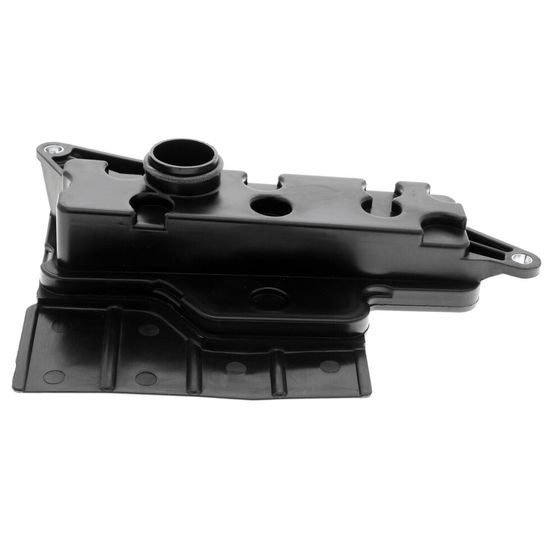
\includegraphics[scale=0.5]{ht_rm.jpg}
    \caption{Hydraulic filter automatic transmission VAICO V70-0613 for Lexus RX \parencite{RM}}
    \label{fig:sparepart}
\end{figure}

\end{appendices}


\end{document}